\documentclass[officiallayout]{tktla} 
%\documentclass[officiallayout,a4frame]{tktla}
\usepackage[latin1]{inputenc}
\usepackage{latexsym}
\usepackage{graphicx}
\usepackage{amsmath}
\usepackage{amssymb}
\usepackage{tikz}
\usetikzlibrary{arrows}
\usetikzlibrary{decorations.pathmorphing}
\usetikzlibrary{fit}					% fitting shapes to coordinates
\usetikzlibrary{backgrounds}
\tikzset{basic/.style={draw,fill=blue!50!green!20,
                       text badly centered,minimum width=3em}}
\tikzset{input/.style={basic,circle}}
\tikzset{weights/.style={basic,rectangle,minimum width=2em}}
\tikzset{functions/.style={basic,circle,fill=blue!50!green!20}}
\def\layersep{2.5cm}

\newcommand{\addsymbol}{\draw (0.5em,0.5em) -- (0,0.5em) -- 
                        (0,-0.5em) --  (-0.5em,-0.5em)
                        (0em,0.75em) -- (0em,-0.75em)
                        (0.75em,0em) -- (-0.75em,0em);}

                        
\newcommand\numberthis{\addtocounter{equation}{1}\tag{\theequation}}    
\newcommand{\wtmat}[2]{W_{#1 #2}}    
%\newcommand{\igate}{\vec{i}}
%\newcommand{\fgate}{\vec{f}}
%\newcommand{\ogate}{\vec{o}}

\newcommand{\igate}{i}
\newcommand{\fgate}{f}
\newcommand{\ogate}{o}
\newcommand{\state}{c}     

\usepackage[ruled,vlined,linesnumbered]{algorithm2e}
\usepackage{algorithmic,color}
\usepackage{amsthm}
\newtheorem{theorem}{Theorem}[section]
\newtheorem{lemma}[theorem]{Lemma}
\newtheorem{cor}[theorem]{Corollary}
\newtheorem{definition}[theorem]{Definition}

\usepackage{algorithmic,color}
\usepackage{float}
\usepackage[super]{nth}


% 
\usepackage{xargs}
\usepackage[colorinlistoftodos,prependcaption,textsize=tiny]{todonotes}
\newcommandx{\unsure}[2][1=]{\todo[linecolor=red,backgroundcolor=red!25,bordercolor=red,#1]{#2}}
\newcommandx{\change}[2][1=]{\todo[linecolor=blue,backgroundcolor=blue!25,bordercolor=blue,#1]{#2}}
\newcommandx{\info}[2][1=]{\todo[linecolor=OliveGreen,backgroundcolor=OliveGreen!25,bordercolor=OliveGreen,#1]{#2}}
\newcommandx{\improvement}[2][1=]{\todo[linecolor=red,backgroundcolor=red!25,bordercolor=red,#1]{#2}}
\newcommandx{\thiswillnotshow}[2][1=]{\todo[disable,#1]{#2}}
%


\title{Deep Learning Algorithms \\ for Control}
\author{Yuan Gao}
\authorcontact{gaoyuankidult@gmail.com\par
  http://www.cs.helsinki.fi/u/yuangao/}
\pubtime{September}{2015}
\reportno{0}
\isbnpaperback{000-00-0000-0}
\isbnpdf{000-00-0000-0}
\issn{1238-8645}
\printhouse{Unigrafia}
\pubpages{7} % --- remember to update this!
% For monographs, the number of the last page of the list of references
% For article-based theses, the number of the last page of the list of
% references of the preamble part + the total number of the pages of
% the original articles and interleaf pages.
\supervisorlist{Dorota Glowacka, University of Helsinki, Finland \newline  Leo K{\"a}rkk{\"a}inen, Nokia Research Center, Finland \newline Honkala Mikko Nokia Research Center, Finland}
\preexaminera{}
\preexaminerb{}
\opponent{}
\custos{}
\generalterms{}
\additionalkeywords{}
\crcshort{A.0, C.0.0}
\crclong{
\item[A.0] Example Category
\item[C.0.0] Another Example
}
\permissionnotice{
}



\begin{document}

\frontmatter
\maketitle
\begin{abstract}
Controlling a complicated mechanical system to perform a certain task, for example, making robot to dance, is a traditional problem studied in the area of control theory. Many successful applications like Google BigDog\cite{Raibert2008} and Google Self-driving car.

However more evidences show that in-cooperating with machine learning techniques in robotics can enable people to get rid of tedious engineering works of adjusting environmental parameters. Many researchers like Jan Peters, Sethu Vijayakumar, Stefan Schaal, Andrew Ng and Sebastian Thrun are the early explorers in this field. Based on the Partial Observable Markov Decision Process(POMDP) reinforcement learning, they contributed theory and practical implementation of several bench marks in this field.

Recently, one sub-field of machine learning called deep learning gained a lot of attention as a method attempting to model high-level abstractions by using model architectures composed by multiple non-linear layers. (for example \cite{Krizhevsky2012}). Several architectures of deep learning networks like deep belief network \cite{Hinton2006}, deep Boltzman machine \cite{Salakhutdinov2009}, convolutional neural network \cite{Krizhevsky2012} and deep de-noising auto-encoder \cite{Vincent2010} have shown its advantages in specific areas. Especially, convolutional neural network, which was invented by Krizhevsky, outperformed all the traditional feature-based machine learning techniques in ImageNet competition.

The main works of deep learning is more related to perception which deals with the problems like Sensor Fusion{OConnor2013}, Nature Language Processing(NLP)\cite{Cho2014} and Object Recognition\cite{Lenz2013}\cite{Hoffman2014}. Although considered briefly in J{\"u}rgen Schmidhuber's team\cite{Mayer2006}, the other area of robotics, namely control, remains more-or-less unexplored in the realm of deep learning.

There are two reasons about why these areas remain unexplored. The first reason is that deep learning method emphasizes on data driving techniques in which we need a lot of data to enable system to find important features whilst we don't have any dataset that can offer large amount of data. The second reason is that applying deep learning techniques requires introducing real robot platform to test the algorithm. This process is hard for researchers as they normally don't have resources for this complicated task.

The main focus of this thesis is to introduce general learning methods for robot control problem with an emphasize on deep learning method. As a consequence, this thesis tries to describe the transitional learning method as well as the emerging deep learning methods for robot control problem.

Ultimately, the author hope the readers of this thesis, even without much background in machine learning or robotics can understand the gists of solution for robot learning problems. 
\end{abstract}

\begin{acknowledgements}
  This is a sample sentence that should look like normal text, and
  this is another. This is a sample sentence that should look like
  normal text, and this is another. This is a sample sentence that
  should look like normal text, and this is another.
\end{acknowledgements}
%Print the glossary

\tableofcontents



\mainmatter
\chapter{Introduction}

Controlling a complicated mechanical system to perform a certain task, for example making robot to dance, is a traditional problem studied in the field of control theory. Many successful applications like Google BigDog\cite{Raibert2008} and Google Self-driving car \cite{guizzo2011google} have been made in accordance to the new theories found in this field.

However more evidences show that in-cooperating with machine learning techniques in robotics can enable people to get rid of tedious engineering works of adjusting environmental parameters. Many researchers like Jan Peters, Sethu Vijayakumar, Stefan Schaal, Andrew Ng and Sebastian Thrun are the early explorers in this field. Based on the Partial Observable Markov Decision Process(POMDP) reinforcement learning, they contributed first several algorithms that enable robot to learn to perform a certain task overtime.

Recently, one sub-field of machine learning called deep learning gained a lot of attention as a method attempting to model high-level abstractions by using model architectures composed by multiple non-linear layers. (for example \cite{Krizhevsky2012}). Several architectures of deep learning networks like deep belief network \cite{Hinton2006}, deep Boltzman machine \cite{Salakhutdinov2009}, convolutional neural network \cite{Krizhevsky2012} and deep de-noising auto-encoder \cite{Vincent2010} have shown its advantages in specific areas. Especially, one of convolutional neural networks, which was invented by Krizhevsky, outperformed all the traditional feature-based machine learning techniques in ImageNet competition.

Based on the two trends we noticed, a natural path of research is to use deep learning methods for controlling movements of robot. Until the end of 2014,  the main works of deep learning are more related to a category of robotics called perception, which deals with problems like Sensor Fusion \cite{OConnor2013}, Nature Language Processing(NLP)\cite{Cho2014} and Object Recognition\cite{Lenz2013}\cite{Hoffman2014}. Although considered briefly in J{\"u}rgen Schmidhuber's team\cite{Mayer2006}, the other area of robotics, namely control, remains more-or-less unexplored in the realm of deep learning.

The researches done in J{\"u}rgen Schmidhuber's team provided several interesting structures that might be potentially useful for robot control. The name of one of these structures is called Long Short Term Memory (LSTM), which is one variation of Recurrent Neural Network(RNN). Several experiments like generating sequences\cite{Graves2013}, speech recognition\cite{Graves2013b} and neural turing machine \cite{Graves2014} show that it has ability of extracting and storing temporal information from data. As a consequence, this specific structure of RNN, with modification, can be applied for control problems of robots.

Currently the main machine learning algorithm used for learning a action is based on reinforcement learning. Specifically, it is based on a category called policy gradient algorithm, which means the algorithm needs to directly search in policy space instead of state-action space. In this framework, there are normally two parts, namely actor part and critic part. Actor part is used for generating different actions based on policy parameters, the critic part is for simulating the environment in order to provide an accurate approximation for the environment. Deep Learning can be used in this case as it is general function approximator and environment is considered as a function that takes several parameters in and output an action.

In thesis, we consider several kind of deep learning models to approximate the environment to reduce the real word samples needed. As a consequence, two major aspects are considered, one main focus of this Thesis is to introduce general learning methods for robot control problem with an emphasize on deep learning method. this thesis tries to describe the transitional learning method as well as the emerging deep learning methods for robot control problem. Another focus of this thesis is to introduce the main contribution of author in this field. With experiments, the author is able to show his own method can outperform the transitional machine learning methods of robot control problems.

\chapter{Reinforcement Learning}

If we would like to discuss what might be the most common way of learning, learning based on interacting with our environment is a natural idea to think about. When we were born in this world, we had no teachers around us. But tens of years passed, we learned to fear, to communicate with others and to write a paper. As a consequence, it is very natural to think that our environment is a great source of information. While playing around with environment, we learn by taking actions and getting reward from it. Now when we cook , when we do exercise, we are fully and acutely aware what will be the response of environment.

The RL is an area that studies the mechanism of the such kind of learning in a computational way. Generally the goal of RL is to find a way of mapping different states with different actions so that we could maximize the reward signals. 

There are two main approaches in area of reinforcement learning, one is based on Markov Decision Process(MDP)\cite{barto1998reinforcement} and another one is recurrent neural network(RNN)\cite{williams1992simple}. Both methods have advantages and drawbacks when applied to robotics.

In the following sections of this chapter, we may consider robot as an agent in all description of related techniques.

\section{Markov Decision Process}
Markov Decision Process (MDP) is a discrete time stochastic control process. We may consider a robot in a state $s$ of discrete state space $S$. The robot can take an action $a$ in all possible action set $A$ resulting in a state $s'$ . We can denote this process as transition function
$P_a(s, s')$ meaning the probability of moving from state
$s$ to state $s'$ through action a. Then after the robot executes action $a$ and results in $s'$ , it will receive a reward $r$ according to reward function denoted as $R_a(s, s ')$. The goal of reinforcement learning is to optimize cumulative reward of whole process. 

The problems of MDP is more clear to researchers as it is based on mathematical formalizations. On one hand, MDP-based methods together with optimization methods such as Gradient Partially Observable Markov Decision Processes (GPOMDP), projection method or nature gradient are state-of-art in robot trajectory learning. On another hand, as data collected from robot is different from normal data, it was pointed out the MDP-based methods suffers several curses\cite{Kober2013}.
\begin{itemize}
\item Curse of Dimensionality
\item Curse of Real-World Samples
\item Curse of Under-Modeling and Model Uncertainty
\item Curse of Goal Specification
\end{itemize}
The data is normally high dimensional, continuous and erroneous data in robot systems. It is considered to be difficult questions to neglect these issues and it is also hard to specify the goal of system i.e. what robot needs to be at last.

\subsection{Partially Observable Markov Decision Process}
A partially observable Markov decision process (POMDP) is a generalization of a Markov decision process (MDP). A POMDP models an agent decision process in which it is assumed that the system dynamics are determined by an MDP, but the agent cannot directly observe the underlying state. Instead, it must maintain a probability distribution over the set of possible states, based on a set of observations and observation probabilities, and the underlying MDP.

The POMDP framework is general enough to model a variety of real-world sequential decision processes. Applications include robot navigation problems, machine maintenance, and planning under uncertainty in general. The framework originated in the operations research community, and was later taken over by the artificial intelligence and automated planning communities.

An exact solution to a POMDP yields the optimal action for each possible belief over the world states. The optimal action maximizes (or minimizes) the expected reward (or cost) of the agent over a possibly infinite horizon. The sequence of optimal actions is known as the optimal policy of the agent for interacting with its environment.

More precisely, the POMDP is a discrete time stochastic control process. We may consider a robot in a state $s_t$ of discrete space $\mathcal{S}$ where t means iteration number. Now the robot can take an action a in all possible action set A resulting in a state $s_{t+1}$. We can denote this process as transition function Ta($s_t$,$s_{t+1}$) meaning the probability of moving from state $s_t$ to state $s_{t+1}$ through action $a$. Then after the robot executes action a and results in st+1, it will receive a reward according to reward function denoted as $R_a(s_t,s_{t+1}$).

Formally, we define MDP as follows:

A Markov decision process is a 4-tuple denoted as ($\mathbb{S}$,$\mathbb{A}$,$T\cdot(\cdot,\cdot)$,$R\cdot(\cdot,\cdot)$)
In this tuple
\begin{itemize}
\item	$\mathbb{S}$ is a finite set of states. It describes all possible states of the space.
\item	$\mathbb{A}$ is a finite set of actions. It describes all possible states that robot can take.
\item	$T\cdot(\cdot,\cdot)$ is a function that takes three arguments. e.g $T_{a_t}(s_t,s_{t+1})$ means probability of transferring from $s_t$ to $s_{t+1}$ with action $a_t$.
\item	$R\cdot(\cdot,\cdot)$ is also a function that takes three arguments. e.g $R_{a_t}(s_t,s_{t+1})$ means reward of transferring from $s_t$ to $s_{t+1}$ with action $a_t$.
\end{itemize}


The main problem of reinforcement learning is to find a policy function $\pi(s) : s \rightarrow a$ to map every state s with action $a$ so that a cumulative reward $R$ is maximized, where $0 \leq \gamma \leq 1$ is a discount factor. As the discount factor generalizes discounted situation and undiscounted situation, it broadens our theory.

\subsection{Markov Decision Process with Continuous States}
Now considering the environment of robots, we need some modifications to original POMDP. First we still assume the process to be discrete time but we consider continuous space $\mathbb{S} \subseteq R^n$ and continuous action set $\mathbb{A} \subseteq R^m$ where $n$ is dimension of space and $m$ is dimension of actions. For initial state $s_0$, we assign a distribution $p(s_0)$ where $s_0 \in \mathcal{S}$. At any state $s_t \in \mathcal{S}$, we have a continuous policy $\pi(a_t|s_t) = p(a_t|s_t,\theta)$ parametrized by $\theta$. Transfer function now also becomes continuous. It is corresponded to a probability distribution $T_{a_t}(s_t,s_{t+1}) = p(s_{t+1}|s_t,a_t)$. After this step is completed, the process will general a reward function $R_{a_t}(s_t,s_{t+1}$) which is defined as $R\cdot(\cdot,\cdot) : S  \times S \times A \rightarrow [0,\inf)$.
After these modifications, we can now formalize continuous MDP.

Continuous Markov Decision Process With Infinite States is a modified version of ordinary POMDP. Mathematically, it is defined as a 5-tuple ($P_{init},S,A,T\cdot(\cdot,\cdot),R\cdot(\cdot,\cdot))$ where in this tuple
\begin{itemize}
\item	$P_{init}$ is a initial distribution of the states.
\item	$\mathbb{S} \subseteq \mathbb{R}^n$ is a infinite set of states. It describes all possible states of the space.
\item	$\mathbb{A} \subseteq \mathbb{R}^m$ is a infinite set of actions. It describes all possible actions of the agent.
\item	$T\cdot(\cdot,\cdot)$ is a function that takes three arguments. e.g $T_{a_t}(s_t,s_{t+1})$ means probability of transferring from st to st+1 with action at.
\item	$R\cdot(\cdot,\cdot)$ is a function that takes three arguments. e.g $R_{a_t}(s_t,s_{t+1})$ means reward of transferring from $s_t$ to $s_{t+1}$ with action at.
\end{itemize}

With this continuous setting, we have objective function defined as follows:

\begin{align}
J(\theta) &= \vec{E_\tau}\{(1-\gamma)\sum_{t=0}^{\infty}\gamma^tR_t|\theta\} \\
&= \int_\mathbb{S}d^\pi(\vec{s})\int_\mathbb{A}\pi(\vec{a}|\vec{s})R(\vec{a}, \vec{s})d\vec{a}d\vec{s}
\end{align}

Where $d^\pi(\vec{s})$ refers to $1 - \gamma^tp(\vec{s} = \vec{s_t})$, $0 \geq \gamma \geq 1$ refers to discount factor and $\pi(\vec{a}|\vec{s})$ is parametrized by $\theta$.
\subsection{Value Functions}
We define two functions to further describe this process. First function is statevalue
function denoted as $V^\pi(\vec{x})$. This means expected value of an agent that follows
an policy of $\pi$ with initial value $\vec{s}$. It characterizes the rewards of following a policy $\pi$. Mathematically, it is defined as:

\begin{equation}
V^\pi(\vec{s}) = \vec{E}_\tau\{\sum_{t=0}^\infty\gamma^tr_t|\vec{s} = \vec{s_0}\}
\end{equation}

where $\tau$ stands for trajectory of agent.
\begin{equation}
Q^\pi(\vec{s}, \vec{a}) = \vec{E}_\tau\{\sum_{t=0}^\infty\gamma^tr_t|\vec{s} = \vec{s_0}, \vec{a} = \vec{a_0}\}
\end{equation}
State-value function only depends on the first state of agent. After that the system
is governed by policy $\pi$. Another value function we need to defines is state-action
value function.
\subsection{Natural Actor Critic Model}
The first thing of demonstrating Natural Actor-Critic is to explain the term. Natural
stands for gradient framework called natural gradient while Actor-Critic means an
iterative method of evaluating and improving objective function.

Robot learning is based on Markov Decision Process with discrete time and continuous
states. The objective function is defined in section Markov Decision Process
by Formula 1. A normal gradient of objective function is defined as :
\begin{equation}
\nabla J(\theta) = \int_\mathbb{S} d^\pi(\vec{s})\int_\mathbb{A}\nabla_\theta \pi(\vec{a}, \vec{s})R(\vec{a}, \vec{s})d\vec{a}d\vec{s}
\label{objective_function}
\end{equation}


Please note $\theta$ is related to $\pi(\vec{a}|\vec{s})$ as it is defined by $\pi(\vec{a}|\vec{s}|\theta)$.

However, here we need to redefine this gradient as vanilla gradient. Pointed out
and nicely presented by Shun-ichi Amari, another kind of gradient called natural
gradient is more efficient in many machine learning application than vanilla gradient.
Mathematically we define following formula as natural gradient:
\begin{equation}
\nabla J(\theta) = G^{-1}\nabla J(\theta)
\end{equation}

Where G is fisher information metrix[].
Fisher information matrix is a matrix defined on Romanian space. This metric
is interesting on several aspects. One of them is that it shows true direction of
a function's steepest direction and on the contrary, the vanilla gradient does not.
The long proof of previous statement is based by showing natural gradient descent
method is fisher efficient. We recommend a further reading on Amari's paper[].

If we rewrite Formula 5 as:

\begin{equation}
\nabla_\theta J(\theta) = \int_\mathbb{S} d^\pi(\vec{s})\int_\mathbb{A}\nabla_\theta \pi(\vec{a}, \vec{s})(Q^\pi(\vec{a}, \vec{s}) -b^\pi(\vec{s}))d\vec{a}d\vec{s}
\end{equation}



Where $Q^\pi(a, s)$ is state-action value function and $b^\pi(x)$ is kind of baseline. Two
papers [] [] demonstrate why $R(s, a)$ is replace by $Q^\pi(a, s) - b^\pi(x)$. It can be
shown that $R(s, a)$ is further approximated as $(\nabla_\theta \log\pi(a,s)^\pi(s))^T \vec{w}$ parametrized by $\vec{w}$.
\section{Reinforcement Learning Methods}

In this section, we introduce common ideas in robotics including temporal difference learning, Episodic learning and policy gradient method.
\subsection{Policy Evaluation}
Policy evaluation is a process that computes state-value function based on a policy $\pi$. Generally, there are three ways of doing policy evaluation. 

The simple every-visit Monte-Carlo method used for evaluating policy is defined as:
\begin{equation}
V^\pi(\vec{s}) \leftarrow V^\pi(s_t) + \gamma (R(s_t) - V(s_t))
\end{equation}
where $V^\pi(s_t)$ is the state-value of state $s_t$, $\gamma$ is discount factor and $R(s_t)$ is the reward of state $s_t$. 

The most well-known one is based on dynamic programming. It computes the best state-value for each state and iteratively update the value to each possible state. This update process can be defined as:
\begin{equation}
V^\pi(\vec{s}) \leftarrow \vec{E}\{r_{s_1} + \gamma V(s_t)\}
\end{equation}

Temporal Difference Learning is another important concept in the area of reinforcement learning. It uses temporal difference information to learn a value function. As a result, it does not need to know every state.(this issue will be address )

As we can see, the simple every-visit Monte-Carlo method only in-cooperate information of current state. However, considering future information may result a better converging rate.

Based on this idea, the simplest TD method(TD(0)) is developed and defined as:
\begin{equation}
V^\pi(\vec{s}) \leftarrow V^\pi(s_t) + \gamma (r_{t+1} + \gamma V(s_{t+1})- V(s_t))
\end{equation}

We may notice that each method requires different kind of data to be used. The simple every-visit Monte-Carlo method only in-cooperate information of current state, so it can be updated just by using the information observed at each state. The TD(0) requires successive two states and dynamic programming requires information of every state.

We may further consider the differences between these three methods based on characteristics they have. Generally, bootstrapping means using estimate of successor state in reinforcement learning. In this case, we can classify these three methods as follows:
\begin{itemize}
\item MC does not bootstrap, as it always uses current state for updating
\item DP bootstraps, as it needs to calculate expectation of all the successive states.
\item TD(0) bootstraps, as it needs to know the state-value function of next state.
\end{itemize}
If we consider whether they use sampling method for not, we also can classify them as following:
\begin{itemize}
\item MC samples
\item DP does not sample
\item TD samples
\end{itemize}

Now I will use TD(0) policy evaluation algorithm as example to show how is policy evaluated.
\newline
\newline
\begin{algorithm}[t]
\caption{Tabular TD(0) policy evaluation algorithm}
\label{algo:adam}
\begin{algorithmic}
 \REQUIRE Policy $\pi$
 Initialize $V(s)$ arbitrarily \;
 \While{until $s$ is terminal(for each episode)}{
  a $\leftarrow$ action given by $\pi$ for state $s$\;
  take action $a$, observe reward $r$ and next state $s'$
  $V^\pi(\vec{s}) \leftarrow V^\pi(s_t) + \gamma (r_{t+1} + \gamma V(s_{t+1})- V(s_t))$
  $s \leftarrow s'$
  }
\end{algorithmic}
\vspace{-0.05in}
\end{algorithm}

\newcommand{\wm}{\widehat{m}_t}
\newcommand{\wv}{\widehat{v}_t}



\subsection{Policy Gradient Methods}
The previous policy evaluation algorithms updates state-value for each state. However, there are also episodic algorithms to evaluate policy based on parameters. In the following text, we are going to introduce policy gradient method for robotics.

Reinforcement learning is probably the most general framework where such robot learning problems can be phrased. Despite the fact that many reinforcement learning algorithm fails to scale where robots have more degrees of freedom, policy gradient methods is one of the exception.

There are several advantages of policy gradient algorithms. According to Jan Peters' paper about policy gradient method\cite{peters2006policy}, firstly the policy representations can be chosen to be meaningful. Secondly the parameters can incorporate previous domain knowledge. The third reason is that policy gradient algorithm has a rather strong theoretical underpinning and additionally, policy gradient algorithms can be used in a model-free fashion.

All these advantages ensures that with only few parameters, robots can learn a decent policy for certain task. Mathematically, policy gradient algorithm tries to optimize policy parameters $\theta \in \mathbb{R}^n$ so that the expected return:
\begin{equation}
J(\theta) = \vec{E}\{\sum_{k=0}^Ha_k r_k\}
\end{equation}
is maximized. where $a_k$ is a weighting factor. It can be set as $\gamma^k$ in discounted case or $\frac{1}{H}$ in average case. The steepest decent algorithm is normally set to be optimization method as for each iteration, we would like to have small changes to the robot system. 
\begin{equation}
\theta_{h+1} = \theta_h + \alpha_h \nabla_\theta J|_{\theta=\theta_h}
\end{equation}
where $\alpha_h$ is learning rate for current updating step $h$.

\section{Classification of the Regarded RL Problems}
Many literatures have pointed out the complexity of RL problem in the area of robotics.\cite{Kober2013}\cite{peters2006policy}. Especially in Kober's paper\cite{Kober2013}, four different aspects were mentioned. He considers these four aspects as four curses for applying RL to robotics. These four curses are curse of High dimensionality, curse of real world samples, curse of under modelling and model uncertainty and curse of goal specification.

\textbf{High-Dimensionality} is the first characteristics considered in the area of robotics. Robot systems normally have many degrees of freedom(DOF), especially in modern anthropomorphic robots. For example, Baxter robot has two arms, each arm has 7 DOF including three pitch degrees and four roll degrees. This continuity makes traditional reinforcement learning fail as many traditional methods are based on discretization of each DOF. If the we discretize $n$ DOFs and discretize each DOF to $m$ states, the total states for the system is $m^n$, which is in inapplicable in most of the cases.

Need of \textbf{Real Samples} is another curse of applying RL to robotics. Robot system inherently interacts with physical system in real world. During test with environment, robot hardware may experience wear and tear. As a consequence, in many cases, this is an expansive process. Despite failure is costly, the test process also requires some kind of supervision from human. For example, we used Baxter to reach certain position as fast as possible. In optimization process, it stucks at a position that is hard to set. If optimization process happens in more complex dynamic environment(e.g. helicopter robot), a supervision process conducted by several human's cooperation is needed. For all these reasons, generating real word samples require different resources and is a expansive process.

\textit{Under-modelling and model uncertainty} is the next problem in robot system. For reducing the cost of real world samples, people build accurate simulators to accelerate learning process. Unfortunately, building such kind of models involves a lot of engineering work, which is also expansive. For small robot system, the simulator can improve learning process to some extend. But if we use simulator to simulate complex system, a small turbulence can cause learned system to diverge from real system.

Last but not the least, \textit{goal specification } means to specify the reward function for the robot system. As in reinforcement learning algorithm, policy optimization process depends on the observing different rewards of two different policies. If a same reward is always received, there is no way of telling which policy is better. In practice, it is surprisingly difficult to specify the reward function of the system. 

These four areas are notorious when people try to apply RL algorithm to robotics. Here we only discuss basic ideas of these problems. However, people who studies applying reinforcement learning in robotics have explored these problems more thoroughly than discussed here. If readers have interest, please refer to paper "Reinforcement learning in robotics: A survey"\cite{Kober2013}

\section{Policy Gradient with Parameter Exploration}
As one of the policy gradient method, Policy Gradient with Parameter Exploration(PGPE) has shown its advantages in several scenarios. This algorithm was developed by Frank Sehnke and described in his paper "Policy Gradient with Parameter Exploration" \cite{sehnke2008policy}. PGPE algorithm follows basic idea of policy gradient algorithm, that is optimizing policy without using value estimation.

\subsection{PGPE algorithm}
As previously mentioned, the policy uses several policy parameters $\vec{\theta}$ to represent policy of the system. In the case of PGPE, the policy is represented as a simple linear model. For formalizing the algorithm, we will uses previous symbols as basis of system.

Considering a robot interacting with environment, at time $t$, the robot is in a state $\vec{s_t}$, making action $\vec{a_t}$ and resulting in state $\vec{s}_{t+1}$ according a stochastic function $\vec{s}_{t+1}\sim p(\vec{s_{t+1}}|\vec{s_t}, \vec{a_t})$. Now with parameter $\vec{\theta}$, the action is defined as $ \vec{a_{t}}\sim p(\vec{a}{t}|\vec{s}_{t},\vec{\theta})$.

In PGPE, the action is determined by $n$ weight matrices($W_i, \forall i \in \{1,2,\cdots, n\}$). Mathematically, the action vector $\vec{a}$ is determined by :
\begin{align}
\vec{a} &= f(\vec{s}) \\
&= \sum_i^n\vec{W_i} \cdot \vec{s}
\end{align}

where $f(\vec{s})$ is defined as $f(\vec{s})$.(sometimes, it is also called a multi-layer linear neural network.).

Each parameter in matrix $W_{ijk}$ is defined by a Gaussian function:
\begin{equation}
W_{ijk} \sim \mathcal{N}(\mu, \sigma^2) = \frac{1}{{\sigma \sqrt {2\pi } }}e^{{{ - \left( {x - \mu } \right)^2 } \mathord{\left/ {\vphantom {{ - \left( {x - \mu } \right)^2 } {2\sigma ^2 }}} \right. \kern-\nulldelimiterspace} {2\sigma ^2 }}}
\label{pgpe_gaussian}
\end{equation}
where $\mu$ and $sigma$ are mean and variance of the algorithm, $W_{ijk}$ means element of $j'th$ row and $k'th$ column of $i'th$ matrix.



The learning process of PGPE is a little bit different than other algorithm. Previously, the objective function is defined according to Formula~\ref{objective_function}. However, in episodic setting, the parameters are updated after each episode, which makes algorithm to depend on sampling of all parameters of this linear neuron network. After sampling parameters for all weights of network, we receive a sequence of all the reward $r_t$ in this episode which results reward of this episode to be $r(h) = \sum_{t=1}^T r_t$. We then modify the algorithm to be:
\begin{equation}
J(\theta) = \int_H p(h|\vec{\theta})r(h)dh
\end{equation}
where $H$ is set of all possible history $h$ of this episode, $h$ is defined as $h = [s_{1:T}, a_{1:T}]$.

Further expanding the formula by using standard identity $\nabla_x y(x) = y(x) \nabla_x \log(x)$:
\begin{equation}
\nabla_{\vec{\theta}} J(\vec{\theta}) = \int_H p(h|\vec{\theta}) \nabla_{\vec{\theta}} \log p(h|\vec{\theta})r(h)dh
\label{stadard_identity_transformation}
\end{equation}
Since the whole process is Markovian process, i.e. we have $ \vec{a_{t}}\sim p(\vec{a}_{t}|\vec{s}_{t},\vec{\theta})$ defined as the transition function. The following property holds: 

\begin{equation}
p(h|\vec{\theta}) = \prod_{i=1}^Tp(\vec{s}_{i+1}|\vec{a}_i, \vec{s}_i)p(\vec{a}_{i}|\vec{s}_{i}, \vec{\theta})p(\vec{s_0})
\label{markov_property}
\end{equation}

\begin{align}
\log(p(h|\vec{\theta})) = \sum_{i=1}^T\log(p(\vec{s}_{i+1}|\vec{a}_i, \vec{s}_i)p(\vec{a}_{i}|\vec{s}_{i}, \vec{\theta})) + \log(\vec{s_0})
\label{log_markov_property}
\end{align}

The term $\nabla_{\vec{\theta}} \log p(h|\vec{\theta})$ in the Formula ~\ref{stadard_identity_transformation} can be rewritten as:
\begin{align}
\nabla_{\vec{\theta}} \log p(h|\vec{\theta})  &= \nabla_{\vec{\theta}} \sum_{i=1}^T\log(p(\vec{s}_{i+1}|\vec{s}_{i}, \vec{\theta})) + \nabla_{\vec{\theta}} \log(\vec{s_0}) \\
&= \nabla_{\vec{\theta}} \sum_{i=1}^T\log(p(\vec{s}_{i+1}|\vec{a}_i, \vec{s}_i)p(\vec{a}_{i}|\vec{s}_{i}, \vec{\theta})) \\
&= \nabla_{\vec{\theta}} \sum_{i=1}^T\log(p(\vec{a}_{i}|\vec{s}_{i}, \vec{\theta}))
\label{expansion_of_log_history}
\end{align}

Then if we substitute the result of Formula~\ref{expansion_of_log_history} to Formula~\ref{stadard_identity_transformation}, we get more convenient form:


\begin{equation}
\nabla_{\vec{\theta}} J(\vec{\theta}) = \int_H p(h|\vec{\theta}) \nabla_{\vec{\theta}} \sum_{i=1}^T\log(p(\vec{a}_{i}|\vec{s}_{i}, \vec{\theta}))r(h)dh
\label{standard_identity_transformation}
\end{equation}

In continuous case, it is impossible to get all the histories for certain set of policy parameters. We need to estimate the gradient based on the samples of this distribution as a result, we further modify our formulas to:
\begin{equation}
\nabla_{\vec{\theta}} J(\vec{\theta}) = \frac{1}{P}\sum_{p=1}^P  \sum_{i=1}^T\nabla_{\vec{\theta}}\log(p(\vec{a_{ip}}|\vec{s_{ip}}, \vec{\theta_p}))r(h_p)
\label{pgpe_policy}
\end{equation}
where, in formula, subscription $p$ means $p'th$ sample of the distribution.

Previously, we discussed that, in PGPE, each parameter of matrices is determined by a Gaussian function as defined in Fomula~\ref{pgpe_gaussian}. As we use weights matrices $W_i$ as hidden policy parameters, the Formula~\ref{standard_identity_transformation} becomes as:
\begin{align*}
\nabla_{\vec{\mu}, \vec{\sigma^2}} J(\vec{\theta}) = \int_H p(h|\vec{\theta}) \nabla_{\vec{\theta}} \sum_{i=1}^T\log(\int_\theta p(\vec{a}_{i}|\vec{s}_{i}, \vec{\theta})p(\vec{\theta}|\vec{\mu},\vec{\sigma^2}))r(h)dh \numberthis \label{standard_identity_transformation_replaced_by_mean_sigma}
\end{align*}

According to this formula, we can make a optimization process for both vectors of means and variances of Gaussian distribution. There are two ways of optimizing the function. One way is to calculate the gradient information of each mean $\mu_i$ and gradient information of each $\sigma$ with respect with respect to $\log(p(\theta| \vec{\mu}, \vec{\sigma^2}))$. From definition of Gaussian function we can get:

\begin{align*}
\nabla_\mu \log(p(\theta| \vec{\mu}, \vec{\sigma^2})) &= \nabla_\mu \log(\frac{1}{\sigma\sqrt{2\pi}}\exp\frac{-(\theta - \mu)}{2\sigma^2}) \\
&= \nabla_\mu -\frac{-(\mu - x)^2}{2\sigma^2} \\
&= \frac{\mu-x}{\sigma^2}   \numberthis \label{gaussian_mean_gradient} 
\end{align*}

and 

\begin{align*}
\nabla_\sigma \log(p(\theta| \vec{\mu}, \vec{\sigma^2})) &= \nabla_\sigma \log(\frac{1}{\sigma\sqrt{2\pi}}\exp\frac{-(\theta - \mu)}{2\sigma^2}) \\
&= -\frac{1}{\sigma} + \frac{(x-\mu)^2}{\sigma^3} \\
&= \frac{(x-\mu)^2 - \sigma^2}{\sigma^3}   \numberthis \label{gaussian_sigma_gradient}
\end{align*}

After getting gradient information of mean $\mu$ and variance $\sigma^2$ of system, we can use method proposed by Williams\cite{williams1992simple}. Instead of knowing exact step size, Williams uses a so-called reference reward to calculate the step size. Formula~\ref{wiliams_update_mean}~\ref{wiliams_update_sigma} shows the updating rules of mean and variances.

\begin{equation}
\Delta \mu = \alpha (r - b)\frac{\mu - x}{\sigma^2}
\label{wiliams_update_mean}
\end{equation}

\begin{equation}
\Delta \sigma = \alpha (r - b)\frac{(x-\mu)^2 - \sigma^2}{\sigma^3}
\label{wiliams_update_sigma}
\end{equation}

This method was influenced by Williams' REINFORCE algorithm as consequence, it inherits the advantages and disadvantages of this algorithm. On one hand, this method has proof of convergence, which means with more trials, this method will finally converge. On the anther hand, this method is also slow and unstable. A better solution based on Simultaneous Perturbation Stochastic Approximation(SPSA) provides fast convergence rate.

This method uses a symmetric sampling process for determining rewards of a specific mean $\mu$ and variance $\sigma$ of random variable. Using SPSA, we first generate small perturbation $\epsilon$ from normal distribution $\mathcal{N}(0, \sigma^2)$. Then we then use two parameters $\vec{\theta}^+ = \vec{\mu} + \vec{\epsilon}$ and $\vec{\theta}^- = \vec{\mu} - \vec{\epsilon}$ for the system to get two rewards $r^+$ and $r^-$. Combining with Formula~\ref{gaussian_mean_gradient} and Formula~\ref{gaussian_sigma_gradient}, we can get gradient information for $\vec{\mu}$ as:
\begin{equation}
\nabla_{\mu_i}J(\vec{\mu}, \vec{\sigma^2}) \approx \frac{\alpha\epsilon(r^+ + r^-)}{\sigma^2}
\end{equation}

Then we use central different method and apply the same step size, then updating rule becomes:
\begin{equation}
\Delta_{u_i} = \alpha \epsilon \frac{(r^+ - r^-)}{2}
\label{sys_update_mu}
\end{equation}

However, we can not use similar method for updating $\sigma$, since the selected two parameters $\theta^+$ and $\theta^-$ have same variances. As a consequence, instead of using information from sample parameter $\epsilon$ along, we also consider the average value of two rewards to update $\sigma$. This updating algorithm is called SyS sampling method in some literature.\cite{sehnke2013efficient}

\begin{equation}
\Delta_{\sigma_i} = \alpha \left(\frac{(r^+ + r^-)}{2} - b) \right)\left(\frac{\epsilon_i^2 - \sigma_i^2}{\sigma_i}\right)
\label{sys_update_sigma}
\end{equation}
where $b$ is baseline and updated before updating hidden policy parameters $\vec{\mu}$ and $\vec{\sigma^2}$.

Formula~\ref{b_update} shows how baseline is updated. Some literature mentioned that variance of the base can affect quite a lot the learning speed of the system.\cite{zhao2011analysis}. But here we only use the simplest way of updating the algorithm.
\begin{equation}
b = 0.1 \cdot b + 0.9 \cdot \frac{r^+ + r^-}{2}
\label{b_update}
\end{equation}


In the following section, we use pseudo code for whole PGPE algorithm.
\newline
\newline
\begin{algorithm}[H]
\caption{Policy Gradient with Parameter Exploration}
 \KwData{The MDP Process Parameters }
 \KwResult{Optimal Policy $\pi*$}
 
 \While{average reward not converged}{
	Get mean $\vec{\mu}$ and variances $\vec{\sigma^2}$ of random variables. \\
	For each parameter, sample $\epsilon$ from Normal Distribution $\mathcal{N}(0, \sigma^2)$ and form a vector $\vec{\epsilon}$.  \\
	Get two parameters using $\vec{\theta}^- = \vec{\mu} - \vec{\epsilon}$, $\vec{\theta}^+ = \vec{\mu} + \vec{\epsilon}$ \\
	Use two parameters as policy parameters, get cumulative reward $r^+$, $r^-$ from system.\\
	Update baseline $b$ of algorithm according to Formula~\ref{b_update}. \\
	Update $\mu$ and $\sigma$ using Formula~\ref{sys_update_mu} and Formula~\ref{sys_update_sigma}. \\
	
  } 
\label{alg:pepg}
\end{algorithm}
 


\chapter{Deep Recurrent Neural Networks}
Recurrent Neural Network(RNN) is a special structure of neural network that has recurrent connections. And further more, deep recurrent neural networks are a neural network models that have more than one hidden layer.  In the following sections of this chapter, we are going to discuss the details of this kind of model. 
\section{Deep Learning and its Recent Advances}
Deep learning attracted a lot of attention since 2006. In year 2006, Geoffrey Hinton, one of the founders of idea deep learning, published a paper called "Reducing the Dimensionality of
Data with Neural Networks"\cite{hinton2006reducing}. In this paper, Hinton and Slakhutdinow showed how a many-layered feedforward neural network can be pre-trained layer by layer. Since this paper, the work "deep learning" become famous in the community. However, before Hinton's work, several deep learning algorithms were developed. One of the initial works belongs to Kunihiko Fukushima who invented a model called Neocognitron in 1980. After that, in 1989, Yann Lecun was able to use an optimization algorithm called back-propagation to train the neuron network. Then Yann Lecun further simplified network to be so-called \textit{Convolutional Neuron Network(CNN)} in 1998. As CNN becomes so successful in the area of computer vision, the deep learning embraced boost after that period. However, other models that has more than one hidden layer is also normally discussed in the context of deep learning. For example, Deep Belief Network (DBN) and Deep Boltzmann Machine(DBM) are not normally considered as neuron network models, but they also have application in the area of computer vision.

\section{Feedforward Neural Networks}
In year 1957, the simplest structure of neural network called perceptron was introduced by Frank Rosenblatt in Conell's Aeronautical Laboratory. This model consists only one cell and multiple connections. Figure~\ref{perceptron} shows the basic structure of perceptron.
\begin{figure}[h!]
  \centering
	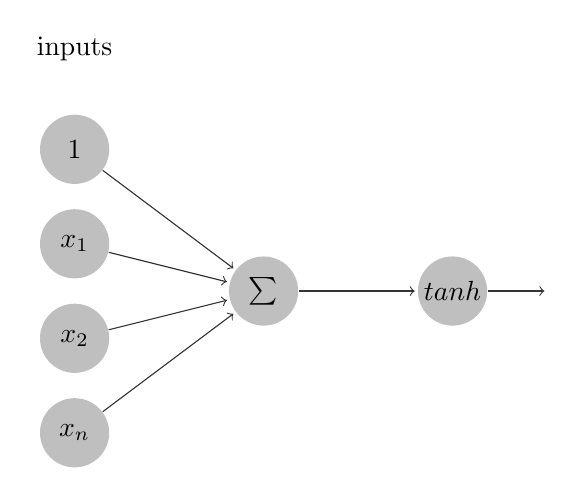
\begin{tikzpicture}[scale=1.2, shorten >=1pt,->,draw=black!80, node distance=\layersep]
    \tikzstyle{every pin edge}=[<-,shorten <=1pt]
    \tikzstyle{neuron}=[circle,fill=black!25,minimum size=25pt,inner sep=0pt]
    \tikzstyle{annot} = [text width=4em, text centered]
            
    
    \node[neuron] (sum) at (4,0) {$\sum$};
    \foreach \h [count=\hi ] in {$x_n$,$x_2$,$x_1$,$1$}{%
          \node[neuron] (f\hi) at (2,\hi*1cm-2.5 cm) {\h};
          \draw[->] (f\hi) -- (sum);
		}

    \node[neuron] (tanh) at (6,0) {};
       \begin{scope}[xshift=6cm,scale=.75]
         \node [] {$tanh$};
       \end{scope}
    \draw[->] (sum) -- (tanh);
    \draw[->] (tanh) -- ++(1,0);
    % Labels
    \node[above=1cm]  at (f4) {inputs};
    \end{tikzpicture}
  \caption{This picture shows the structure of perceptron, the i'th input is shown as $x_i$ and corresponded weights are denoted as $w_i$. There is also a bias term name $b$ connected to cell, which, with a addition function, generates the output.}\label{proceptron}
\end{figure}

The formula of representing input and output is defined as:

\begin{equation}
y = \vec{w}\cdot\vec{x} + b
\end{equation}

If we consider $b$ also as one of the inputs, then the formula can be defined as:

\begin{equation}
y = \vec{w}_{new}\cdot\vec{x}_{new}
\end{equation}\label{pronceptron_formula}

where $ \vec{w}_{new} = [\vec{w};b] $ and $\vec{x} = [\vec{x};1]$.

This simple structure was considered promising initially from several points of view. But after further investigation, the perceptron was proven that it can not classify many non-linear classes of patterns. However, its discovery leads to a field of research called neural networks in area artificial intelligence. As a consequence, since 1957, people started trying different methods for modifying this model to adapt to different problems. One important modification is to add a non-linear transformation function to the system i.e. after getting $y$ from Formula\ref{pernceptron_formula}, we use a function like tanh to get a new $\hat{y}$ to ensure the output is restricted in a range. Anther important modification of the system is to stack many perceptrons together to build a large and complex model for the classification purpose. This kind of networks is normally called Feed-forward Neural Networks(FFNN) as information send to this system is propagated only from lower layer to higher layer. Figure~\ref{feedforward_nn} shows the structure of FFNN system.



\begin{figure}[h!]
  \centering

	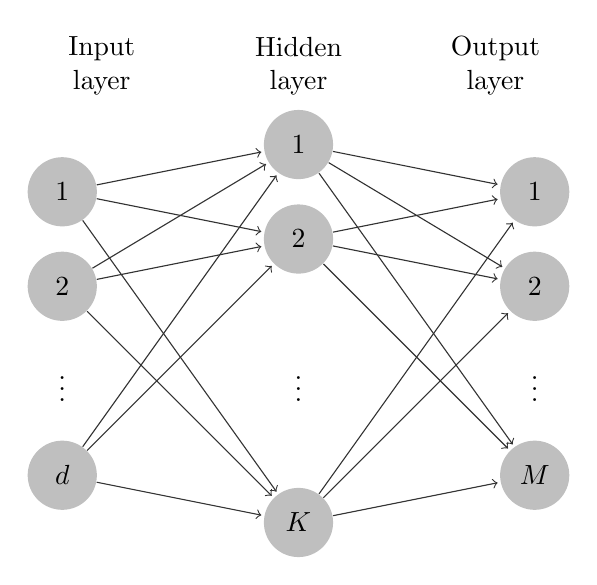
\begin{tikzpicture}[scale=1.2, shorten >=1pt,->,draw=black!80, node distance=\layersep]
    \tikzstyle{every pin edge}=[<-,shorten <=1pt]
    \tikzstyle{neuron}=[circle,fill=black!25,minimum size=25pt,inner sep=0pt]
    \tikzstyle{annot} = [text width=4em, text centered]

    % Draw the input layer nodes
    \foreach \name / \y in {1/1,2/2,$d$/4}
    % This is the same as writing \foreach \name / \y in {1/1,2/2,3/3,4/4}
        \node[neuron] (I-\name) at (0,-\y) {\name};
    \node (I-3) at (0,-3) {\vdots};

    % Draw the hidden layer nodes
    \foreach \name / \y in {1/1,2/2,$K$/5}
        \path[yshift=0.5cm]
            node[neuron] (H-\name) at (\layersep,-\y cm) {\name};
    \node (H-3) at (\layersep,-3) {\vdots};

    \foreach \name / \y in {1/1.5,2/2.5,$M$/4.5}
        \path[yshift=0.5cm]
            node[neuron] (O-\name) at (2*\layersep,-\y cm) {\name};
    \node (O-3) at (2*\layersep,-3) {\vdots};

    % Connect every node in the input layer with every node in the
    % hidden layer.
    \foreach \source in {1,2,$d$}
        \foreach \dest in {1,2,$K$}
            \path (I-\source) edge (H-\dest);
    
   
    % Connect every node in the hidden layer with the output layer
    \foreach \source in {1,2,$K$}
        \foreach \dest in {1,2,$M$}
            \path (H-\source) edge (O-\dest);

    % Annotate the layers
    \node[annot,above of=H-1, node distance=1cm] (hl) {Hidden layer};
    \node[annot,left of=hl] {Input layer};
    \node[annot,right of=hl] {Output layer};
	\end{tikzpicture}
  \caption{This picture shows the structure of Feed-forward Neural Network. There are three layers in this network, namely the input layer, hidden layer and the output layer. For connections from input layer to hidden layer, the i'th input is shown as $x_i$ and corresponded weights of hidden neuron $j$ is denoted as $W_{ij}$.}\label{feedforward_nn}
\end{figure}

The formula describing the each layer is then defined as:

\begin{equation}
f(\vec{x}) = \sigma(W\vec{x})
\end{equation}
where $\sigma(\cdot)$ is a nonlinear function.(e.g. tanh)

\section{Recurrent Neural Networks}
The Recurrent Neural Networks(RNN) contains at least one neuron that has at least one recurrent connection i.e. a connection that connects to itself or to lower layer. This special structure makes memory cell to be internal memory which enables network to memories the change of sequential data. Unlike the feed-forward neural network, the recurrent neural network is used for predicting next data point.

\begin{figure}[h!]
  \centering
  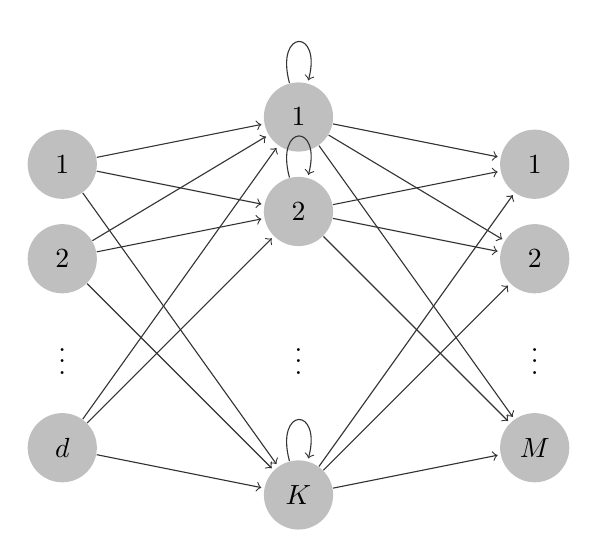
\begin{tikzpicture}[scale=1.2, shorten >=1pt,->,draw=black!80, node distance=\layersep]
    \tikzstyle{every pin edge}=[<-,shorten <=1pt]
    \tikzstyle{neuron}=[circle,fill=black!25,minimum size=25pt,inner sep=0pt]
    \tikzstyle{annot} = [text width=4em, text centered]

    % Draw the input layer nodes
    \foreach \name / \y in {1/1,2/2,$d$/4}
    % This is the same as writing \foreach \name / \y in {1/1,2/2,3/3,4/4}
        \node[neuron] (I-\name) at (0,-\y) {\name};
    \node (I-3) at (0,-3) {\vdots};

    % Draw the hidden layer nodes
    \foreach \name / \y in {1/1,2/2,$K$/5}
        \path[yshift=0.5cm]
            node[neuron] (H-\name) at (\layersep,-\y cm) {\name};

    \node (H-3) at (\layersep,-3) {\vdots};

    \foreach \name / \y in {1/1.5,2/2.5,$M$/4.5}
        \path[yshift=0.5cm]
            node[neuron] (O-\name) at (2*\layersep,-\y cm) {\name};
    \node (O-3) at (2*\layersep,-3) {\vdots};

    % Connect every node in the input layer with every node in the
    % hidden layer.
    \foreach \source in {1,2,$d$}
        \foreach \dest in {1,2,$K$}
            \path (I-\source) edge (H-\dest);
    
    % Connect hidden layer to hidden layer
    \foreach \source in {1,2,$K$}
		\path (H-\source) edge [loop above] (H-\source);
    
    
    % Connect every node in the hidden layer with the output layer
    \foreach \source in {1,2,$K$}
        \foreach \dest in {1,2,$M$}
            \path (H-\source) edge (O-\dest);
\end{tikzpicture}
  \caption{This picture shows the structure of recurrent neural network. There are two layers in this networ namely input layer and hidden layer, the first layer contains notes connected to the input data. The second layer stores information and also forwards information to next layer. The cell in the hidden layer has a connection to itself which means the information stored in the cell at time $t-1$ also influences the information stored in the cell at time $t$}\label{feedforward_nn}
\end{figure}

\subsection{Finite Unfolding in Time}
When considering the structure of neural network, people normally application Finite Unfolding in Time for RNN. It means to introduce another dimension for RNN. In this way, the recurrent connection can be dealt with more easily.  In the following section, we will use a simple example for explaining this idea. The model we are going to use contains one input neuron, one hidden neuron and one output neuron. See Figure~\ref{simple_rnn} for reference.



\begin{figure}[h!]
\centering
\tikzstyle{background}=[rectangle,fill=gray!10,inner sep=0.5cm, rounded corners=5mm]
\begin{tikzpicture}[>=latex,text height=1.5ex,text depth=0.25ex]
	\tikzstyle{neuron}=[circle,fill=black!25,minimum size=25pt,inner sep=0pt]
	\tikzstyle{cdots_neuron}=[circle,fill=gray!10,minimum size=25pt,inner sep=0pt]
    % "text height" and "text depth" are required to vertically
    % align the labels with and without indices.
  
  % The various elements are conveniently placed using a matrix:
  \matrix[row sep=0.6cm,column sep=0.5cm] {
    % First line: Control input
    		&
        \node (x_t-1) [neuron]{$\vec{x}_{t-1}$}; &
        &
        \node (x_t)   [neuron]{$\vec{x}_t$};     &
		&
		\node (cdots_x)   [cdots_neuron] {$\cdots$};
													&
        	&
        	\node (x_n-1)   [neuron] {$\vec{x}_{n-1}$};
													&
        	&         	
        \node (x_n) [neuron]{$\vec{x}_{n}$}; &

        \\
        % Third line: State & state transition matrix
		\\
		&
        \node (s_t-1) [neuron] {$\vec{s}_{t-1}$}; &
		&
        \node (s_t)   [neuron] {$\vec{s}_t$};     &
        
		&
		\node (cdots_s)   [cdots_neuron] {$\cdots$};
													&
        	&
        	\node (s_n-1)   [neuron] {$\vec{s}_{n-1}$};
													&
        	&        		
        \node (s_n) [neuron] {$\vec{s}_{n}$}; &
		\\
		\\

        % Fifth line: Measurement
        &
        \node (o_t-1) [neuron] {$\vec{o}_{t-1}$}; &
        &
        \node (o_t)   [neuron] {$\vec{o}_t$};     &
        	&
		\node (cdots_o)   [cdots_neuron] {$\cdots$};
													&
        	&
        	\node (o_n-1)   [neuron] {$\vec{o}_{n-1}$};
													&
        	&         	
        \node (o_n) [neuron] {$\vec{o}_{n}$}; &
        \\
    };
    
    % The diagram elements are now connected through arrows:
    \path[->]
    	    (x_t-1) edge (s_t-1)
        (x_t) edge (s_t)
        (x_n-1) edge (s_n-1)
        (x_n) edge (s_n)
        	        	
        (s_t-1) edge (s_t)
        (s_t) edge (cdots_s)  
        
        (cdots_s) edge (s_n-1)
    	    (s_t-1) edge (o_t-1)
        (s_t) edge (o_t)
        (s_n-1) edge (o_n-1)
        (s_n) edge (o_n)
        ;
    
    % Now that the diagram has been drawn, background rectangles
    % can be fitted to its elements. This requires the TikZ
    % libraries "fit" and "background".
    % Control input and measurement are labeled. These labels have
    % not been translated to English as "Measurement" instead of
    % "Messung" would not look good due to it being too long a word.
    \begin{pgfonlayer}{background}
        \node [background,
                    fit=(x_t-1) (x_n),
                    label=left:Inputs:] {};
        \node [background,
                    fit=(s_t-1) (s_n),
                    label=left:Hidden States:] {};
        \node [background,
                    fit=(o_t-1) (o_n),
                    label=left:Outputs:] {};
    \end{pgfonlayer}
\end{tikzpicture}
  \caption{This picture shows the structure of a simple RNN. It contains three layers i.e. one input layer, one hidden layer and one output layer.}\label{simple_rnn}
\end{figure}

In this figure, we mark input layer as $\vec{x}$, hidden layer as $\vec{s}$ and output layer as $\vec{o}$.

The basics idea of unfolding RNN in time is to copy RNN several times and connect them in a chronological order. If the connection is recurrent, then the connection should be connect to the same neuron of next time step.Figure~\ref{unfolded_simple_rnn} illustrates the model of unfolding simple RNN  for three time steps.

\begin{figure}[h!]
  \centering
% The input, state transition, and measurement matrices
% are represented by gray squares.
% They have a smaller minimal size for aesthetic reasons.
\tikzstyle{matrx}=[rectangle,
                                    thick,
                                    minimum size=1cm,
                                    draw=gray!80,
                                    fill=gray!20]


% Everything is drawn on underlying gray rectangles with
% rounded corners.
\tikzstyle{background}=[rectangle,
                                                fill=gray!10,
                                                inner sep=0.5cm,
                                                rounded corners=5mm]

\begin{tikzpicture}[>=latex,text height=1.5ex,text depth=0.25ex]
	\tikzstyle{neuron}=[circle,fill=black!25,minimum size=25pt,inner sep=0pt]
    % "text height" and "text depth" are required to vertically
    % align the labels with and without indices.
  
  % The various elements are conveniently placed using a matrix:
  \matrix[row sep=0.6cm,column sep=0.5cm] {
    % First line: Control input
    		&
        \node (x_t-1) [neuron]{$\vec{x}_{t-1}$}; &
        &
        \node (x_t)   [neuron]{$\vec{x}_t$};     &
        &
        \node (x_t+1) [neuron]{$\vec{x}_{t+1}$}; &

        \\
        % Third line: State & state transition matrix
		\\
		&
        \node (s_t-1) [neuron] {$\vec{s}_{t-1}$}; &
		&
        \node (s_t)   [neuron] {$\vec{s}_t$};     &
		&
        \node (s_t+1) [neuron] {$\vec{s}_{t+1}$}; &
		\\
		\\

        % Fifth line: Measurement
        &
        \node (o_t-1) [neuron] {$\vec{o}_{t-1}$}; &
        &
        \node (o_t)   [neuron] {$\vec{o}_t$};     &
        &
        \node (o_t+1) [neuron] {$\vec{o}_{t+1}$}; &
        \\
    };
    
    % The diagram elements are now connected through arrows:
    \path[->]
    	    (x_t-1) edge (s_t-1)
        (x_t) edge (s_t)
        (x_t+1) edge (s_t+1)
        	        	
        (s_t-1) edge (s_t)
        (s_t) edge (s_t+1)  
        
    	    (s_t-1) edge (o_t-1)
        (s_t) edge (o_t)
        (s_t+1) edge (o_t+1)
        ;
    
    % Now that the diagram has been drawn, background rectangles
    % can be fitted to its elements. This requires the TikZ
    % libraries "fit" and "background".
    % Control input and measurement are labeled. These labels have
    % not been translated to English as "Measurement" instead of
    % "Messung" would not look good due to it being too long a word.
    \begin{pgfonlayer}{background}
        \node [background,
                    fit=(x_t-1) (x_t+1),
                    label=left:Inputs:] {};
        \node [background,
                    fit=(s_t-1) (s_t+1),
                    label=left:Hidden States:] {};
        \node [background,
                    fit=(o_t-1) (o_t+1),
                    label=left:Outputs:] {};
    \end{pgfonlayer}
\end{tikzpicture}
  \caption{This picture contains model that unfolds a simple RNN described in Figure\ref{simple_rnn} in abitary $n$ time steps. In this figure, $x_t$ represents input layer at time $t$, $s_t$ representes the hiddent states at time $t$ and $o_t$ representes output layer at time $t$.}\label{unfolded_simple_rnn}
\end{figure}

The finite unfolding technique transforms a neural network with recurrent connection to a network that is easier to compute gradients. It is also easy for us to write this neural network's expression.

\begin{equation}
\vec{s_{t}} = \sigma(W\vec{x}_t + B\vec{s}_{t-1})\label{internal_state_fomula}
\end{equation}
Where $\vec{s_t}$ is the value of hidden state at time $t$ and $B$ is the weight matrix for updating hidden state information from time $t-1$ to $t$.


\subsection{Overshooting}
Considering that we only one time series, the task for RNN is to predict next data point based on previous data we have. There are two steps for solving this problem. First we need to copy the data into two set and shift the input by one to produce output. It is illustrated as shown in Figure~\ref{overshot_rnn}.

\begin{figure}[h!]
  \centering
\tikzstyle{matrx}=[rectangle,thick,minimum size=1cm,draw=gray!80,fill=gray!20]


% Everything is drawn on underlying gray rectangles with
% rounded corners.
\tikzstyle{background}=[rectangle,fill=gray!10,inner sep=0.5cm,rounded corners=5mm]
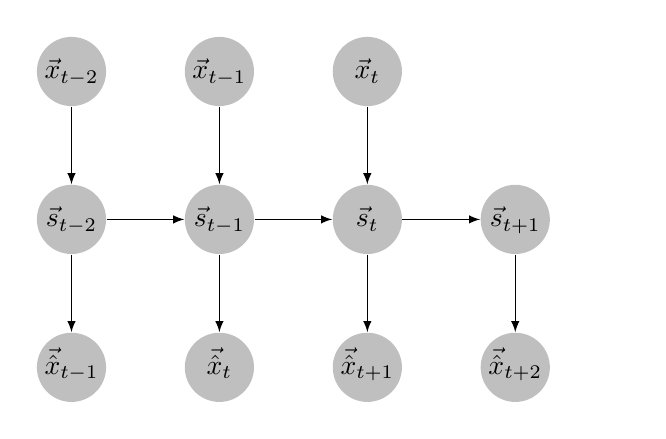
\begin{tikzpicture}[>=latex,text height=1.5ex,text depth=0.25ex]
	\tikzstyle{neuron}=[circle,fill=black!25,minimum size=25pt,inner sep=0pt]
    % "text height" and "text depth" are required to vertically
    % align the labels with and without indices.
  
  % The various elements are conveniently placed using a matrix:
  \matrix[row sep=0.5cm,column sep=0.5cm] {
    % First line: Control input
		\node (x_t-2) [neuron]{$\vec{x}_{t-2}$}; &
    		&
        \node (x_t-1) [neuron]{$\vec{x}_{t-1}$}; &
        &
        \node (x_t)   [neuron]{$\vec{x}_t$};     &
        &
        & &

        \\
        % Third line: State & state transition matrix
		\\
		\node (s_t-2) [neuron]{$\vec{s}_{t-2}$}; &
		&
        \node (s_t-1) [neuron] {$\vec{s}_{t-1}$}; &
		&
        \node (s_t)   [neuron] {$\vec{s}_t$};     &
		&
        \node (s_t+1) [neuron] {$\vec{s}_{t+1}$}; &
		\\
		\\
		
        \node (hat_x_t-1) [neuron]{$\vec{\hat{x}}_{t-1}$}; &
        &
        \node (hat_x_t) [neuron] {$\vec{\hat{x}}_{t}$}; &
        &
        \node (hat_x_t+1)   [neuron] {$\vec{\hat{x}}_{t+1}$};     &
        &
        \node (hat_x_t+2) [neuron] {$\vec{\hat{x}}_{t+2}$}; &
        \\
    };
    
    % The diagram elements are now connected through arrows:
    \path[->]
    		(x_t-2) edge (s_t-2)
    	    (x_t-1) edge (s_t-1)
        (x_t) edge (s_t)
        	  
	    (s_t-2) edge (s_t-1)        	        	
        (s_t-1) edge (s_t)
        (s_t) edge (s_t+1)  

		(s_t-2) edge (hat_x_t-1)       
    	    (s_t-1) edge (hat_x_t)
        (s_t) edge (hat_x_t+1)
        (s_t+1) edge (hat_x_t+2)
        ;
    
    % Now that the diagram has been drawn, background rectangles
    % can be fitted to its elements. This requires the TikZ
    % libraries "fit" and "background".
    % Control input and measurement are labeled. These labels have
    % not been translated to English as "Measurement" instead of
    % "Messung" would not look good due to it being too long a word.

\end{tikzpicture}
  \caption{This figure isllustrates in a predictive model made by RNN, how does it generate $\hat{x_t}$ based on previous data. After using all training example, the model lacks input data. Then the neural caluclation of hidden defined as $\vec{s_{t}} = \sigma(W\vec{x_t} + B\vec{s_{t-1}}))$ becomes $\vec{s_{t}} = \sigma(B\vec{s_{t-1}})$}\label{overshot_rnn}
\end{figure}

Last training step takes input $\vec{x}(t-2)$, $\vec{x}(t-1)$, $\vec{x}(t)$ as input and produce $\vec{x}(t-1)$, $\vec{x}(t)$, $\vec{x}(t+1)$ as outputs. However it is very difficult to predict value at time t+2 as we don't have information of $\vec{x}(t+1)$. According to the Fomula~\ref{internal_state_fomula}, the input is set to $\vec{0}\quad \forall t > T$ then we get:

\begin{equation}
\vec{s_{t}} = \sigma(B\vec{s_{t-1}})\label{overshot_formula}
\end{equation}

As a consequence, the output defined as $\vec{x_{t+1}} = A\vec{s_{t}}$ becomes the prediction for next value. This phenomenon is called overshooting.
\subsection{Dynamical Consistency}

Dynamical consistency is kept by introducing the output of last time step to input of current time step. Figure~\ref{series_prediction_rnn} illustrates how is it done through the modification of structure.

\begin{figure}[h!]
  \centering
  \tikzstyle{matrx}=[rectangle,
                                    thick,
                                    minimum size=1cm,
                                    draw=gray!80,
                                    fill=gray!20]

\tikzstyle{dashed_matrx}=[rectangle,
                                    thick,
                                    dashed,
                                    minimum size=1cm,
                                    draw=gray!80,
                                    fill=gray!20]

\tikzstyle{background}=[rectangle,
                                                fill=gray!10,
                                                inner sep=0.5cm,
                                                rounded corners=5mm]
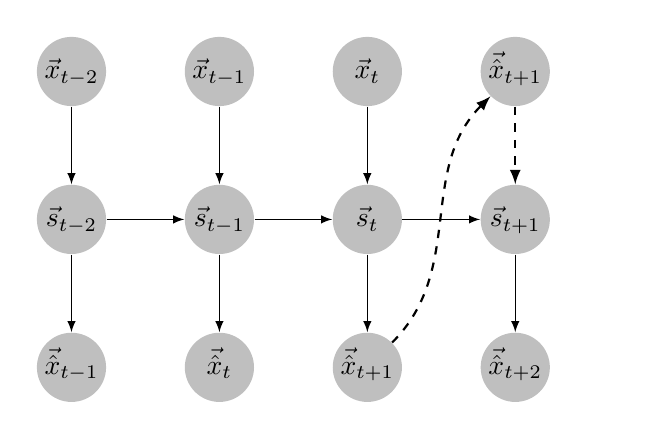
\begin{tikzpicture}[>=latex,text height=1.5ex,text depth=0.25ex]
    % "text height" and "text depth" are required to vertically
    % align the labels with and without indices.
  \tikzstyle{neuron}=[circle,fill=black!25,minimum size=25pt,inner sep=0pt]
  \tikzstyle{dashed_neuron}=[circle, dashed, fill=black!25,minimum size=25pt,inner sep=0pt]
  % The various elements are conveniently placed using a matrix:
  \matrix[row sep=0.5cm,column sep=0.5cm] {
    % First line: Control input
		\node (x_t-2) [neuron]{$\vec{x}_{t-2}$}; &
    		&
        \node (x_t-1) [neuron]{$\vec{x}_{t-1}$}; &
        &
        \node (x_t)   [neuron]{$\vec{x}_t$};     &
        &
        \node (x_t+1)   [dashed_neuron]{$\vec{\hat{x}}_{t+1}$}; 	  & 
        &

        \\
        % Third line: State & state transition matrix
		\\
		\node (s_t-2) [neuron]{$\vec{s}_{t-2}$}; &
		&
        \node (s_t-1) [neuron] {$\vec{s}_{t-1}$}; &
		&
        \node (s_t)   [neuron] {$\vec{s}_t$};     &
		&
        \node (s_t+1) [neuron] {$\vec{s}_{t+1}$}; &
		\\
		\\
		
        \node (hat_x_t-1) [neuron]{$\vec{\hat{x}}_{t-1}$}; &
        &
        \node (hat_x_t) [neuron] {$\vec{\hat{x}}_{t}$}; &
        &
        \node (hat_x_t+1) [neuron] {$\vec{\hat{x}}_{t+1}$};     &
        &
        \node (hat_x_t+2) [neuron] {$\vec{\hat{x}}_{t+2}$}; &
        \\
    };
    
    % The diagram elements are now connected through arrows:
    \path[->]
    		(x_t-2) edge (s_t-2)
    	    (x_t-1) edge (s_t-1)
        (x_t) edge (s_t)
        (x_t+1) edge[thick,dashed] (s_t+1)
        	  
	    (s_t-2) edge (s_t-1)        	        	
        (s_t-1) edge (s_t)
        (s_t) edge (s_t+1)  

		(s_t-2) edge (hat_x_t-1)       
    	    (s_t-1) edge (hat_x_t)
        (s_t) edge (hat_x_t+1)
        (s_t+1) edge (hat_x_t+2)
        (hat_x_t+1) edge[thick, dashed, -latex, out=45,in=225] (x_t+1)
        ;
    
    % Now that the diagram has been drawn, background rectangles
    % can be fitted to its elements. This requires the TikZ
    % libraries "fit" and "background".
    % Control input and measurement are labeled. These labels have
    % not been translated to English as "Measurement" instead of
    % "Messung" would not look good due to it being too long a word.

\end{tikzpicture}
  \caption{This picture contains model for predicting data for time series. For the first unfolded structure of neural network, the data of series at time t-2 is fed to the network and we expect data at time t-1 are predict by the network.}\label{series_prediction_rnn}
\end{figure}

By remembering all the parameters in the network and unfold in time for several steps, the recurrent neural network is able to predict the next data point in the sequence. The relationship between input and output is listed as follows:

\begin{align}
\vec{s_{t}} &= \sigma(W\vec{x_t} + B\vec{s_{t-1}}) \\
\vec{x_{t+1}} &= A\vec{s_{t}}
\end{align}

where $A$ means weight matrix of internal states to output states.


To sum up, the dynamics of system becomes as follows.

\begin{align}
\vec{s_{t}} &= \sigma(W\vec{x_t} + B\vec{s}_{t-1}) \quad \forall t \leq T \label{training_rnn}\\ 
\vec{s_{t}} &= \sigma(W\vec{\hat{x}}_t + B\vec{s}_{t-1}) \quad \forall t > T \label{prediction_rnn}\\
\vec{o_{t+1}} &= A\vec{s_{t}} \quad \forall t \leq T - 1 \label{train_output}\\
\vec{\hat{x}}_{t+1} &= A\vec{s_{t}}  \quad \forall t > T - 1  \label{train_prediction}
\end{align}

Formula~\ref{training_rnn} shows how are values of internal states updated at the training stage. Formula~\ref{prediction_rnn} shows how are values of output data predicted after training stage. Formula~\ref{train_output} shows how outputs generated after training stage. Formula~\ref{train_prediction} shows how outputs predicted after training stage. The overall goal of the system is to minimize the different between the output and predicted output for all time series. Mathematically, it is defined as:

\begin{equation}
J = \sum_{i=1}^{T}\vec{o}_{t} - \vec{y}_{t}
\end{equation}

If we assume each input and output has N data points, then the cost becomes:

\begin{equation}
J = \sum_{i=1}^{T}\sum_{n=1}^{N}o^n_{t} - y^n_{t}
\end{equation}

The main goal of function is to minimize the cost over function parameters defined in the network.(See section ~\ref{training_rnn} for more reference.)

\section{Universal Approximation}
It has been proven that multi-layer feed-forward neural networks are universal approximators by Hornik in 1989. Similar works have also been mentioned by Cybenko and Funahashi in the same year. In this work, Hornik continued work of Minskey and Papert about two layers network. Minkey and Papert proved that two-layer neural networks are not able to approximate functions that do not belong to a special class. Then 	by adding a third layer, the neural network is able to approximate different functions.

Details of approximation theory of multi-layer neuron network is governed by Stone-Weierstrass theorem. This theory states that every continuous function defined on a closed interval $[a, b]$ can be uniformly approximated by a polynomial function. As a result, it also proves that a neuron network with more than one hidden layer can approximate any function.

RNN, as special model of neuron network model also follows Stone-Weierstrass theorem. Herrn Anton Maximilian Schafer proved that RNN is also a universal approximator.


\section{Learning Long-Term Dependencies}

Long-term dependences is an important concept in control. Some states of the system can be crucial to the system. They might influence the future behaviour of the system in many ways. For example, in the T maze example(see Figure~\ref{tmaze} for reference), the decision at the turning  point is essential for the system. As the behaviour is totally different after turning point, a long term memory is important in this case.
\begin{figure}[h!]
\centering
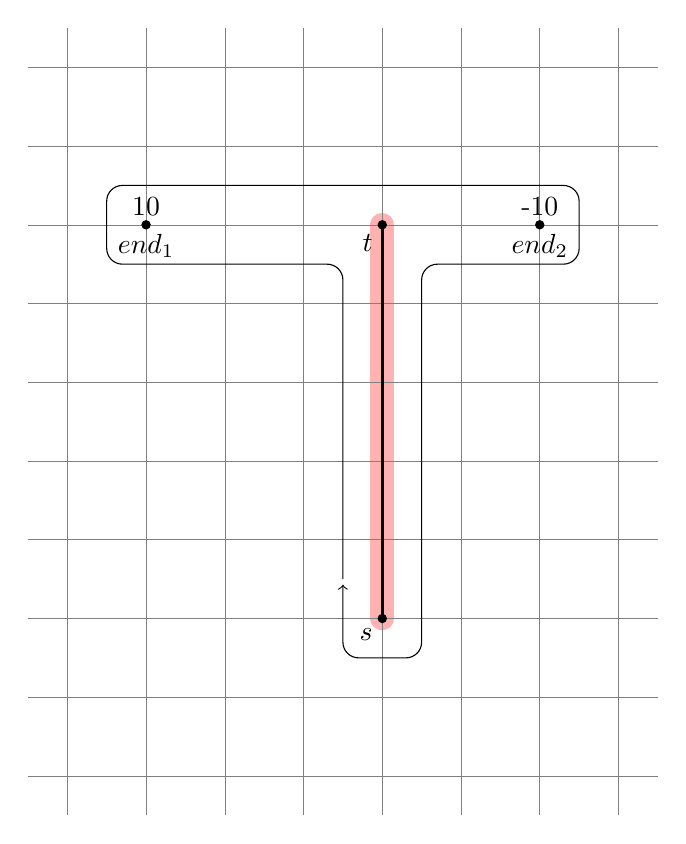
\begin{tikzpicture}
  \draw[line width=0.3cm,color=red!30,cap=round,join=round] (2,0)--(2,5);
  \draw[help lines] (-2.5,-2.5) grid (5.5,7.5);
  \draw[very thick] (2,-0)-- (2,5);
  \draw[below left] (2,0) node(s){$s$};
  \draw[below left] (2,5) node(t){$t$};
  
  \draw[below] (-1,5) node(end_1){$end_1$};
  \draw[below] (4,5) node(end_2){$end_2$};
   
  \draw[above] (-1,5) node(end1_text){10};
  \draw[above] (4,5) node(end1_text){-10};
  
  \fill (2,0) circle (0.06cm) (2,5) circle (0.06cm);
  \fill (-1,5) circle (0.06cm) (4,5) circle (0.06cm);
  \draw[->,rounded corners=0.2cm,shorten >=2pt]
    (1.5,0.5)-- ++(0,1)-- ++(0,1)-- ++(0,1)-- ++(0,1)-- ++(-1,0)-- ++(-1,0)-- ++(-1,0)-- ++(0,1)
    -- ++(1,0)-- ++(1,0)-- ++(1,0)-- ++(1,0)-- ++(1,0)-- ++(1,0)-- ++(0,-1)-- ++(-1,0)-- ++(-1,0)
    -- ++(0,-1)-- ++(0,-1)-- ++(0,-1)-- ++(0,-1)-- ++(0,-1)-- ++(-1,0)-- ++(0,1);
\end{tikzpicture}

\caption{This picture shows the example of a T maze problem. State $s$ is the starting state. It needs to go to end of the maze to terminate the process. At the end state 1, it get 10 reward from the environment and at the end state 2, it get a punishment from the environment. The agent wants to maximize the reward it gets from environment, as a consequence, the turning state $t$ is important for it.}\label{tmaze}
\end{figure}


Traditional RNN has several problems. One famous problem is that it suffers exploding and vanishing gradient problem as when RNN is unfolded in time, it becomes neurally deep. For example, The gradient becomes very small as we back-propagate it to first few layers. Although, there are methods like policy gradient and optimal ordered problem solver that can solve this problem, some specially designed RNN also has this ability.

However, traditional RNNs suffered exploding or vanishing gradient problem. As training of RNN normally requires unfolding of the network in time. Comparing with FFNN, it is naturally deep and as a result, the gradient becomes smaller and smaller after several iterations of computing gradient.

Soon after people discovered this problem, several new structures of RNN were developed for keeping long-term memory. Long Short Term Memory(LSTM) is one of them.

LSTM is normally treated as a hidden layer in a neural network system. It normally adds some extra components in network. More specifically, it has input connections, three gates, outputs connection. A more illustrative example is shown in the following Figure~\ref{lstm}.

\begin{figure}[h!]
  \centering
  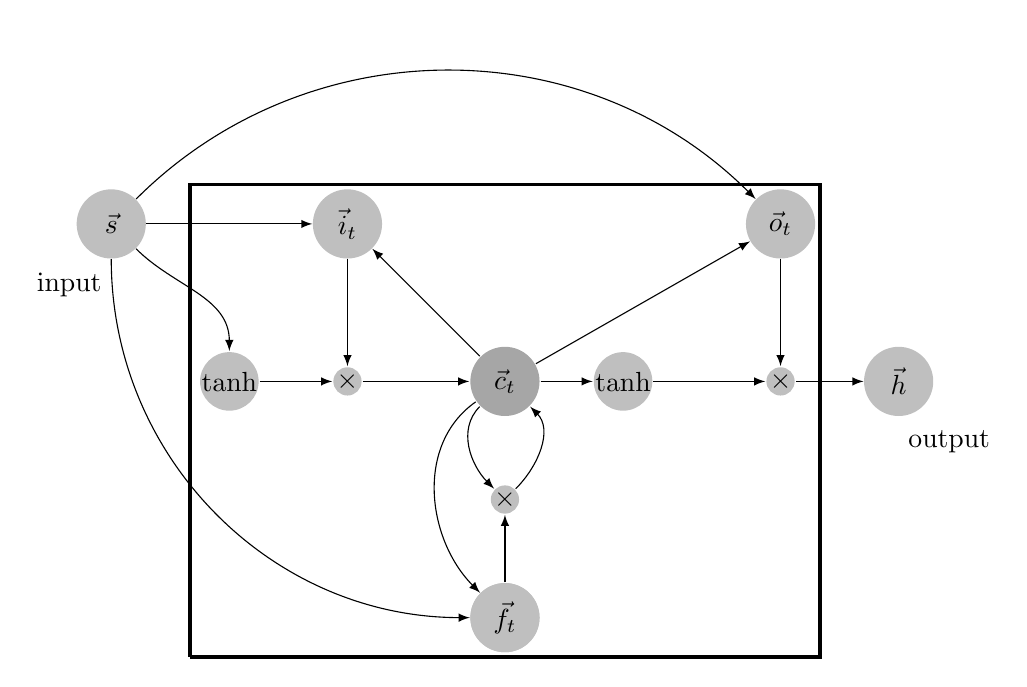
\begin{tikzpicture}
  \coordinate (A) at (-2,0);
  \coordinate (B) at (6,0);  
  \coordinate (C) at (6,6);
  \coordinate (D) at (-2,6);

  
  \tikzstyle{neuron}=[circle,fill=black!25,minimum size=25pt,inner sep=0pt];
  \tikzstyle{memory_cell}=[circle, thick, fill=black!35,minimum size=25pt,inner sep=0pt];
  \tikzstyle{multiplier}=[circle, thick, fill=black!25, minimum size=10pt,inner sep=0pt];
  \tikzstyle{nonlinearity}=[circle, thick, fill=black!25,minimum size=15pt,inner sep=0pt];

  \node (input) at (-3, 5.5) [neuron]{$\vec{s}$};
  \draw[below left] (-3, 5) node {input};
  
  \node (output) at (7, 3.5) [neuron]{$\vec{h}$};
  \draw[below right] (7, 3) node {output};  
   
  \node (input_gate) at (0, 5.5) [neuron]{$\vec{i}_t$};
  \node (output_gate) at (5.5, 5.5) [neuron]{$\vec{o}_t$};
  \node (forget_gate) at (2, 0.5)[neuron]{$\vec{f}_t$};
  
  \node (forget_gate) at (2, 0.5)[neuron]{$\vec{f}_t$};
  
  \node (multiplier_1) at (0, 3.5)[multiplier]{$\times$};
  \node (multiplier_2) at (5.5, 3.5)[multiplier]{$\times$};
  \node (multiplier_3) at (2, 2)[multiplier]{$\times$};
  
  \node (memory) at (2, 3.5)[memory_cell]{$\vec{c}_t$};
  
  \node (nonlinearity_1) at (-1.5, 3.5)[nonlinearity]{$\tanh$};
  \node (nonlinearity_2) at (3.5, 3.5)[nonlinearity]{$\tanh$};
  
  \draw[very thick] (A)--(B)--(C)--(D)--(A);

  \draw[->] (input) edge[-latex, out=0, in=180](input_gate);
  \draw[->] (input) edge[-latex, out=45, in=135](output_gate);
  \draw[->] (input) edge[-latex, out=-90, in=180](forget_gate);
  \draw[->] (input) edge[-latex, out=-45, in=90](nonlinearity_1);

  \draw[->] (multiplier_2) edge[-latex](output);
  
  \draw[->] (memory) edge[-latex](input_gate);
  
  \draw[->] (input_gate) edge[-latex](multiplier_1);
  \draw[->] (nonlinearity_1) edge[-latex](multiplier_1);
  
  \draw[->] (multiplier_1) edge[-latex](memory);
  \draw[->] (multiplier_3) edge[-latex, out=45,in=-45] (memory);
  
  \draw[->] (memory) edge[-latex, out=-135,in=135] (multiplier_3);
  \draw[->] (forget_gate) edge[-latex](multiplier_3);
  
  \draw[->] (memory) edge[-latex, out=-145,in=135](forget_gate);  

  \draw[->] (memory) edge[-latex](nonlinearity_2);
  
  \draw[->] (output_gate) edge[-latex](multiplier_2);
  \draw[->] (nonlinearity_2) edge[-latex](multiplier_2);  

  \draw[->] (memory) edge[-latex] (output_gate);
	
\end{tikzpicture}
  \caption{This figure shows the basic strucuture of LSTM. In the middel, there is the memory cell which keeps the information of the data sequence. Around it, there are three gates, namely input gate, output gate and foget gate. Each of them gets information from the input and controls the updatting rule of memory cell. At the left side, there is input connection. On right side, there is output connection of this layer.}\label{lstm}
\end{figure}

The idea of LSTM is relatively straight forward. The memory cell stores information of the sequential data. Gates try remember when and how much the information  in memory cell should be updated. Mathematically, the process is defined by Formulas from \ref{igate_math} to \ref{output_math}.

\begin{align}
\vec{\igate}_t &= \sigma\left(\wtmat{x}{\igate} \vec{x}_t + \wtmat{h}{\igate} \vec{h}_{t-1} + \wtmat{\state}{\igate} \vec{\state}_{t-1}  + \vec{b}_\igate\right) \label{igate_math}\\
\vec{\fgate}_t &= \sigma\left(\wtmat{x}{\fgate} \vec{x}_t + \wtmat{h}{\fgate} \vec{h}_{t-1} + \wtmat{\state}{\fgate} \vec{\state}_{t-1} + \vec{b}_\fgate \right) \label{fgate_math}\\
\vec{\state}_t &= \vec{\fgate}_t \vec{\state}_{t-1} + \vec{\igate}_t \tanh \left(\wtmat{x}{\state} \vec{x}_t + \wtmat{h}{\state} \vec{h}_{t-1} + \vec{b}_\state\right) \label{cell}\\
\vec{\ogate}_t &= \sigma\left(\wtmat{x}{\ogate} \vec{x}_t + \wtmat{h}{\ogate} \vec{h}_{t-1} + \wtmat{\state}{\ogate} \vec{\state}_{t} + \vec{b}_\ogate\right)\label{ogate_math}\\
\vec{h}_t &= \vec{\ogate}_t \tanh(\vec{\state}_t) \label{output_math}
\end{align}

Formula~\ref{igate_math} describes the update rule of input gate. It takes the output of last time step of system $h_{t-1}$, the input for current time step $\vec{x}_t$, the memory cell value of the last time step $\vec{c}_{t-1}$ and bias term $\vec{b}_t$ in to its updating rule. Similarly Formula~\ref{fgate_math} to Formula~\ref{output_math} also use these parameters to update its value. Generally , input gate controls information flow in to memory cell, forget gate controls information flow out of the system and output gate controls how information can be translated to output. These three gates form a path of remembering the long term dependence of the system.

After knowing the how parameters in LSTM are updated, the next step is to determine what kind of optimization process should be applied to the network so that it can be optimized easily.

\section{Training of RNN}\label{training_rnn}
After getting data and designing the structure of network, the next important step is to train the network to model the data we have and also to predict next point in the data sequence. The main goal of training is to minimize the cost of objective function between expected outcome and real outcome. As a result, predicting data based on data we have.

\subsubsection{Backpropagation}
Backpropagation is an algorithm that uses gradient information of the network to update the parameters of the system. The basic idea of this algorithm is to first use output of the system $\vec{o}$ and real data $\vec{y}$ to compute the error $J(\theta) = |\vec{o} - \vec{y}|_2$. Then the algorithm uses this information to calculate $\Delta W_h$ of the hidden layer and further calculate $\Delta W_i$ of input layer. Normally this algorithm also uses a parameter $\alpha$ to decide the step size of the algorithm, which make the real updating rule of the parameters to be $W_ {t+1}=\alpha \cdot \Delta W_t + W_t$
\begin{algorithm}[ht]
\caption{\emph{Backpropagation}}
\label{algo:backpropagation}
\begin{algorithmic}
\REQUIRE $\alpha$: Stepsize
\REQUIRE $\delta$: Threshold
\REQUIRE $W_{1\ldots n}$: Randomly initialized weights
\WHILE{$J \leq \delta$}
\STATE $\vec{o} = net\left(\vec{i}\right)$
\STATE $J(W_{1,\ldots,n}) = |\vec{o} - \vec{y}|_2$
\STATE $ \nabla W_i = \frac{\partial J(W_i)}{\partial W_i}, \forall i \in \{1, \ldots, n\}$
\STATE $ W_i = \alpha \cdot \nabla W_i  + W_i, \forall i \in \{1, \ldots, n\}$
\ENDWHILE
\RETURN $\theta_t$ (Resulting parameters)
\end{algorithmic}
\vspace{-0.05in}
\end{algorithm}

The basic gradient descent approach (and its backpropagation algorithm implementation) is notorious for slow convergence, because the learning rate $\alpha$ must be typically chosen small to avoid instability. Many speed-up techniques are described in the literature. As a first order method, dynamic learning rate adaptation schemes is sometimes used to system. It has complexity $O(TM)$, where T is number of epoch and M is number of connections. Sometime people also use second-order gradient descent techniques, which exploit curvature of the gradient but have epoch complexity $O(TM^2)$. These two classes of methods are main streams in the optimization problem. 

However, with using these methods, the system still suffers local error minimum, which means the optimization stacks at some local minimum and can not get out. For this particular problem, there are normally three ways of solving it.

\begin{itemize}
\item adding noise
\item repeating the entire learning from different initial weight settings
\item using task-specific prior information to start from an already plausible set of weights
\end{itemize}

In the following section, we will briefly introduce two methods that are able to optimize the LSTM in practice. One of them is called Nesterov's Accelerated Gradient and another of them is called Adam.

\subsection{Shared Weight Extended Backpropagation}

Training algorithm of recurrent neural network, called shared weight backpropagation, is introduced from feed-forward neural network backpropagation. For simplicity of this algorithm, we first consider a simple feed-forward neural network defined as:

\begin{equation}
y = \sigma(W_h\sigma(W_i\vec{x}))
\end{equation}

This network only contains three layers including input layer, hidden layer and output layer. Input layer has $n_i$ input neurons, $h_i$ hidden neuron and output layer has $n_o$ output neurons. The data we have is a list of input-output pairs. Now we add one more recurrent connection to add recurrent connection weights $W_t$. The formula of describing the one step of the system becomes like Formula~\ref{one_step_rnn_bp}.

\begin{equation}
y = \sigma(W_h(\sigma(W_i\vec{x})+\sigma(W_{t}\vec{s}_{t-1}))) \label{one_step_rnn_bp}
\end{equation}

When we unfold the network in time more then one steps, the system will become like illustrated by Figure~\ref{shared_bp}. In the figure, all connections of the network share the same weights. In this case, we need to decide how could we update the weight of each parameter otherwise if we update the each parameter according to gradient information, all updates will eliminate each other.
\begin{figure}[h!]
  \centering
% The input, state transition, and measurement matrices
% are represented by gray squares.
% They have a smaller minimal size for aesthetic reasons.
\tikzstyle{matrx}=[rectangle,
                                    thick,
                                    minimum size=1cm,
                                    draw=gray!80,
                                    fill=gray!20]


% Everything is drawn on underlying gray rectangles with
% rounded corners.
\tikzstyle{background}=[rectangle,
                                                fill=gray!10,
                                                inner sep=0.5cm,
                                                rounded corners=5mm]

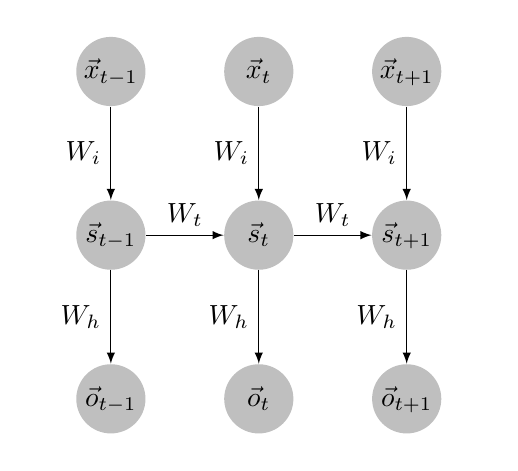
\begin{tikzpicture}[>=latex,text height=1.5ex,text depth=0.25ex]
	\tikzstyle{neuron}=[circle,fill=black!25,minimum size=25pt,inner sep=0pt]
    % "text height" and "text depth" are required to vertically
    % align the labels with and without indices.
  
  % The various elements are conveniently placed using a matrix:
  \matrix[row sep=0.6cm,column sep=0.5cm] {
    % First line: Control input
    		&
        \node (x_t-1) [neuron]{$\vec{x}_{t-1}$}; &
        &
        \node (x_t)   [neuron]{$\vec{x}_t$};     &
        &
        \node (x_t+1) [neuron]{$\vec{x}_{t+1}$}; &

        \\
        % Third line: State & state transition matrix
		\\
		&
        \node (s_t-1) [neuron] {$\vec{s}_{t-1}$}; &
		&
        \node (s_t)   [neuron] {$\vec{s}_t$};     &
		&
        \node (s_t+1) [neuron] {$\vec{s}_{t+1}$}; &
		\\
		\\

        % Fifth line: Measurement
        &
        \node (o_t-1) [neuron] {$\vec{o}_{t-1}$}; &
        &
        \node (o_t)   [neuron] {$\vec{o}_t$};     &
        &
        \node (o_t+1) [neuron] {$\vec{o}_{t+1}$}; &
        \\
    };
    
    % The diagram elements are now connected through arrows:
    \path[->]
    	    (x_t-1) edge node[left]{$W_i$} (s_t-1)
        (x_t) edge node[left]{$W_i$}(s_t)
        (x_t+1) edge node[left]{$W_i$}(s_t+1)
        	        	
        (s_t-1) edge node[above]{$W_{t}$}(s_t)
        (s_t) edge node[above]{$W_{t}$}(s_t+1)  
        
    	    (s_t-1) edge node[left]{$W_{h}$} (o_t-1)
        (s_t) edge node[left]{$W_{h}$} (o_t)
        (s_t+1) edge node[left]{$W_{h}$} (o_t+1)
        ;
\end{tikzpicture}
  \caption{This figure shows the RNN network when it is unfolded in time, each paramer is copy several times. The unfolded network shares all the weights of original RNN.}\label{shared_bp}
\end{figure}

\begin{algorithm}
 \KwData{List of input-output pairs }
 \KwResult{return the network with parameters $W$}
 initialize network weights (often small random values)\;
 \While{training example ex}{
        prediction = neural-net-output(network, ex)\;
        actual = teacher-output(ex)\;
        compute error (prediction - actual) at the output units\;
        compute $\Delta W$ for all weights from hidden layer to input layer\;
        update network weights \;
        until all examples classified correctly or another stopping criterion satisfied
 }
 \caption{Backpropagation for two layers feed-forward neural network.}\label{backpropagation}
\end{algorithm}

The key element in this algorithm is the updating rule of the system. Based on 




Optimizing neuron network is not a simple task. People tried different method since perceptron was introduced. However, only until the back-propagation algorithm was introduced, the neuron network models have a role in the machine learning field. Currently, back-propagation has become standard of training neuron network and many optimization algorithms for neuron network are based on that. In the following section, I will first describe the basic back propagation algorithm and them describe two optimization methods I used in the experiments. One of them is call \textit{Nesterov's Accelerated Gradient}(NAG) and another of them is called \textit{Adam}. 


\subsubsection{Nesterovs Accelerated Gradient}
Nesterov's Accelerated Gradient is sometimes called Nesterov's momentum. Here momentum refers to Classic Momentum(CM) method which is a technique to accelerate the standard gradient descent algorithm. Let recall the original gradient descent algorithm, which update parameters based on a step size $\alpha$ and gradient information of objective function. Formula~\ref{normal_gradient_descent}
\begin{equation}
\Delta_\theta = -\alpha \nabla_{\vec{\theta}} f(\vec{\theta})
\label{normal_gradient_descent}
\end{equation}
CM method adds a momentum coefficient $\mu$ to system and use this parameter to include a momentum-like behaviour in the optimization process. The updating rule for parameters become influenced by the momentum as shown in Formula~\ref{class_momentum}.

\begin{equation}
\widetilde{\Delta}_{\theta t} =  \mu \widetilde{\Delta}_{\theta {t-1}}  -\alpha \nabla_{\vec{\theta}} f(\vec{\theta})
\label{class_momentum}
\end{equation}

NAG, like CM algorithm, is a first order optimization algorithm. For a general smooth(non-strongly) convex functions and deterministic gradient, NAG has a convergence rate of $O(\frac{1}{T^2})$, where $T$ means optimization steps. Comparing convergence rate of $O(\frac{1}{T})$ for CM, it is exponentially faster. The updating rule for NAG is show in Formula~\ref{nag} .In fact, there is not much difference between CM and NAG. 

\begin{equation}
\widetilde{\Delta}_{\theta t} =  \mu \widetilde{\Delta}_{\theta {t-1}}  -\alpha \nabla_{\vec{\theta}} f(\vec{\theta} + \mu \widetilde{\Delta}_{\theta {t-1}})
\label{nag}
\end{equation}

\subsubsection{Adam}
Adam is a first-order gradient-based algorithm \cite{kingma2014adam} invented by 	Diederik Kingma and Jimmy Ba in 2015. It combines ideas of RMSProp\cite{tieleman2012lecture} and AdaGrad\cite{duchi2011adaptive}. Algorithm~\ref{algo:adam} shows the each step of this algorithm.

\begin{algorithm}[ht]
\caption{\emph{Adam}, $g^2_t$ indicates the elementwise square $g_t \odot g_t$. Good default settings for the tested machine learning problems are $\alpha=0.001$, $\beta_1=0.9$, $\beta_2=0.999$, $\epsilon = 10^{-8}$ and $\lambda = 1-10^{-8}$.}
\label{algo:adam}
\begin{algorithmic}[h]
\REQUIRE $\alpha$: Stepsize
\REQUIRE $\beta_1,\beta_2\in [0,1)$, $\lambda\in[0,1]$ : Exponential decay rates for the moment estimates
%\REQUIRE ${ (1-\beta_1)^2 / \sqrt{1-\beta_2}} < 1$: Constraint from convergence analysis
\REQUIRE $f(\theta)$: Stochastic objective function with parameters $\theta$
\REQUIRE $\theta_0$: Initial parameter vector
\STATE $m_0 \gets 0$ (Initialize initial \nth{1} moment vector)
\STATE $v_0 \gets 0$ (Initialize initial \nth{2} moment vector)
\STATE $t \gets 0$ (Initialize timestep)
\WHILE{$\theta_t$ not converged}
\STATE $t \gets t + 1$
\STATE $\beta_{1,t} \gets \beta_1\lambda^{t-1}$ (Decay the first moment running average coefficient)
\STATE $g_t \gets \nabla_{\theta} f_t(\theta_{t-1})$ (Get gradients w.r.t. stochastic objective at timestep $t$)
\STATE $m_t \gets \beta_{1,t} \cdot m_{t-1} + (1-\beta_{1,t}) \cdot g_t$ (Update biased first moment estimate)
\STATE $v_t \gets \beta_2 \cdot v_{t-1} + (1-\beta_2) \cdot g^2_t$ (Update biased second raw moment estimate)
\STATE $\wm \gets m_t / (1-\beta_1^t)$ (Compute bias-corrected first moment estimate)
\STATE $\wv \gets v_t / (1-\beta_2^t)$ (Compute bias-corrected second raw moment estimate)
\STATE $\theta_t \gets \theta_{t-1} - \alpha \cdot \wm / (\sqrt{\wv} + \epsilon)$ (Update parameters)
\ENDWHILE
\RETURN $\theta_t$ (Resulting parameters)
\end{algorithmic}
\vspace{-0.05in}
\end{algorithm}
Adam's parameters are invariant to rescaling of the gradient. By using statistical information,it step sizes are approximately bounded by hyper-parameters, which enables it to perform better by using step size annealing. For more reference, you could look at the paper made by Kingma, Diederik and Ba\cite{kingma2014adam}.
 
\chapter{Prior Arts of Combining Deep Neuron Network and RL}
Different research groups have tried different methods for combining deep neuron networks with reinforcement learning. The first thoughts turned out to be using neuron network as a general controller. In the early work applying neuron network to control algorithm, several algorithms using neuron network were proposed including Explanation-Based Neural Network Learning\cite{thrun1996explanation} and Neural networks for self-learning control systems. \cite{nguyen1990neural}. These early initiatives provide information about how could one formulate a 
\section{Deep Q Network}
Deep Q Network is a network proposed by Google's deep learning group. It creates a direction of combining Convolutional Neuron Network with Q learning algorithm\cite{mnih2013playing}\cite{mnih2015human}. 
That is actually the first 



\chapter{Experiment}

\section{Cart-pole Balancing}
Cart-pole balancing problem has been a basic test problem in the control theory. It considers a physical agent that tries to balance a pole attached to it. Figure~\ref{cart_pendulum} illustrates the situation of the system. The system consist several states including the position $s$ and velocity $\dot{s}$ of the cart, angle $\theta$ and angular velocity $\dot{\theta}$ of the pole. The task involved in this process is to apply a suitable force to enable the system to balance the pole $L$ so that the angle $\theta$ and position of cart $s$ are kept in a range.
\begin{figure}[ht]
\centering
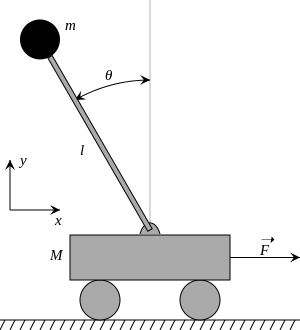
\includegraphics[scale=0.5]{cart_pendulum}
\caption{This figure shows the cart-pole balancing system. A force $\vec{F}$ is exerted on the cart C with mass $M$ to balance a pole l that also has length $l$ attached to it. A mass $m$ is attached on pole L. The system has four states including point of the system $s$, velocity of the system $\dot{s}$, angel between pole L and normal $\theta$ and angular acceleration $ \dot{\theta}$. When force $\vec{F}$ is exerted on cart C, the L will also have a force on the point of attachment with cart and the task is to provide forces that can keep position of cart as well as angel $\theta$ between pole and normal in a range of allowed values(e.g. $s \in [-4,4]$, $\theta \in [-0.2, 0.2]$)}
\label{cart_pendulum}
\end{figure}

Based on the information we have about the system, we can write the Lagrangian of system. 
\begin{equation}
L = \frac{1}{2} M \dot{s}^2 + \frac{1}{2} m v_m^2 - mgl\cos(\theta)
\end{equation}
where, in this case, the $v_m$ is the speed of the a mass attached to pole $L$.
We infer from system 

\begin{equation}
v_m^2=\left(	\frac{d}{dt}(x - l\sin(\theta) \right)^2 + \left(\frac{d}{dt}(l\cos(\theta)\right)^2
\end{equation}
Then it can be further simplified as 	
\begin{equation}
v_m^2=\dot{s}^2-2l\dot{x}\dot{\theta} \cos(\theta) + l^2\dot{\theta}^2
\end{equation}

Following the definition of Lagrange the equations of motion are defined as:
\begin{align}
\frac{d}{ds}\frac{\partial L}{\partial \dot{s}} - \frac{\partial L}{\partial s} = F \\
\frac{d}{dt}\frac{\partial L}{\partial \dot{\theta}} - \frac{\partial L}{\partial \theta} = 0
\end{align}
If we substitute the Lagrangian into system, we find the two equations of motion become like 
\begin{align}
(M + m)\ddot{s} - 	ml\ddot{\theta} \cos(\theta) + \frac{1}{2}ml^2\dot{\theta}^2 - mgl\cos(\theta) = F \\
l\ddot{\theta} - g\sin(\theta) = \ddot{s} \cos(\theta)
\end{align}
Traditional control algorithms like proportional-integral-derivative controller (PID) control can solve problem with high frequency loop. Although it is an entrance level problem in control theory and also in reinforcement learning, it is also a basic example to test effectiveness of the algorithm.

We used this model for testing the basic performance of the policy gradient algorithm. In this case, the policy algorithm also needs to take into account the states and evaluate the action. During the process, it needs to update it policy parameters from experience gained from its failures.

Normally the process' reward is calculated by simulator during the training of actor network. However, at mean time, we also learn a model that can also predict the reward and action according to the previous we gathered.
\subsection{System Implementation}

The system is implemented using a several libraries of python including Pybrain, Theano and nntools to provide easy use of the testing process. 

Pybrain is library developed by IDSIA \cite{pybrain2010jmlr} in order to offer flexible, easy-to-use yet still powerful algorithms for machine learning tasks. It is excellent for reinforcement learning researchers as it separates reinforcement learning into three parts namely, environment, agent and task. In this way, the library actually builds a framework for further development.

Theano is a GPU-based computational library for implementing deep learning algorithm. It has complete support for different deep learning structures including Convolutional Neuron Networks(CNN), Deep Blief Network(DBN) or Restricted Boltzmann Machine(RBM). It builds itself on scipy, which is a scientific computing library of python and numpy, which is a numerical computation library of python. This enables the library to provide the best computation performance for the system. It also uses Cuda-toolkit to support GPU-based computation, which ensures the nvidia-based system can have best performance.

nntools is library built on Theano. It provides modularized APIs for different deep learning architectures.

We use these libraries to build reinforcement learning platform. Following the the MDP process, we need to figure out four important elements of MDP process, namely, ($\mathbb{S}$,$\mathbb{A}$,$T\cdot(\cdot,\cdot)$,$R\cdot(\cdot,\cdot)$). $\mathbb{S}$ is the set of all states of the system. Each state $s \in \mathbb{S}$ contains four physical parameters including $s$ position of the cart, $\dot{s}$ velocity of the cart, $\theta$ angle of pole, $\dot{\theta}$ angular velocity of the pole. The action $a \in \mathbb{A}$ is decided by policy parameters and current states. Transition probability $T$ is decided by the physical system and reward function $R$ is defined as following:

\begin{equation}
    R(s,\theta, t)= 
\begin{cases}
    0,				& \text{if} |s|\leq 0.05, |\theta| \leq 0.05, t \leq 200\\
    -1,              & 2.4 \geq |s|\geq 0.05, 0.7 \geq |\theta| \geq 0.05, t \leq 200\\
    -2 \cdot (200 - t), 		& \text{otherwise}
\end{cases}
\end{equation}
Where $t$ is the time steps that system has been running.

\subsection{Experiment Result}
The result of the algorithm for solving a cart-pole balancing problem is great. Within 300 trials, it can find best policy parameters for the system. However, it needs a little bit longer to get best average rewards. Figure~\ref{cart_pole_pgpe_benchmark} shows the performance of the PGPE algorithm on cart-pole balancing problem.
\begin{figure}[H]
\centering
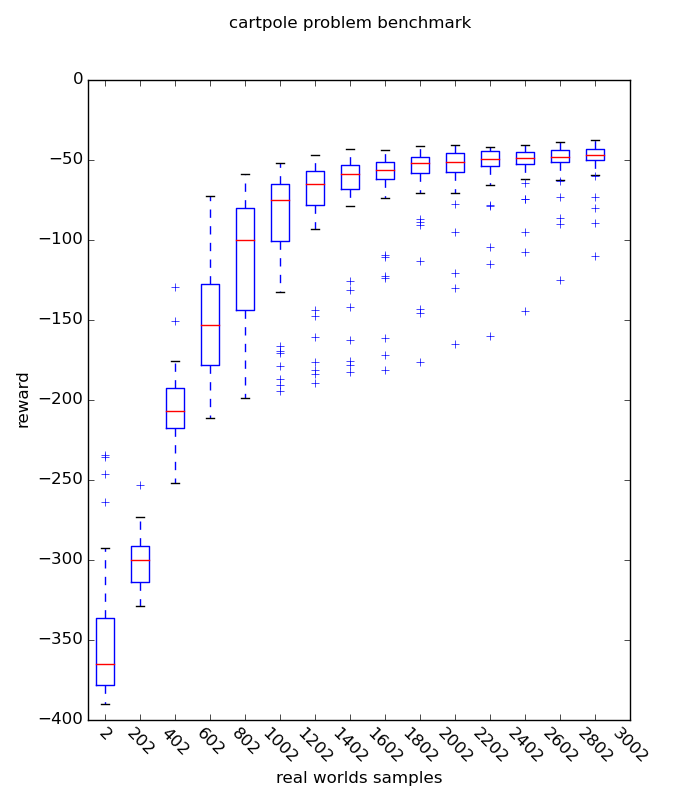
\includegraphics[scale=0.7]{model_pgpe_benchatk}
\caption{This figure shows the result of benchmark of cart-pole balancing problem. The x-axis represents the real word samples needed for training and the y-axis represents the average reward of 50 trials.}
\label{cart_pole_pgpe_benchmark}
\end{figure}


\section{Baxter Robot Learning a Action}
Baxter robot is a research robot developed by rethink company(as shown in Figure~\ref{baxter}).It has two arms, two gripper and animated face. In this experiment, we will use its arms and gripper to learn to perform a certain wood stacking task. In following sections, we will discuss how is this experiment implemented.
\begin{figure}[h]
\centering
\includegraphics[scale=0.17]{baxter}
\label{baxter}
\caption{This figure shows a baxter research robot. We can see that it has a face and two arms.}
\end{figure}
\subsection{System Implementation}
Each arm of Baxter contains seven degrees of freedom including four roll degrees of freedom $s_0$, $e_0$, $w_0$ and $w_2$, three pitch degrees of freedom $s_1$ , $e_1$ $w_1$. The detail of the information is presented in picture.
\begin{figure}[h]
\centering
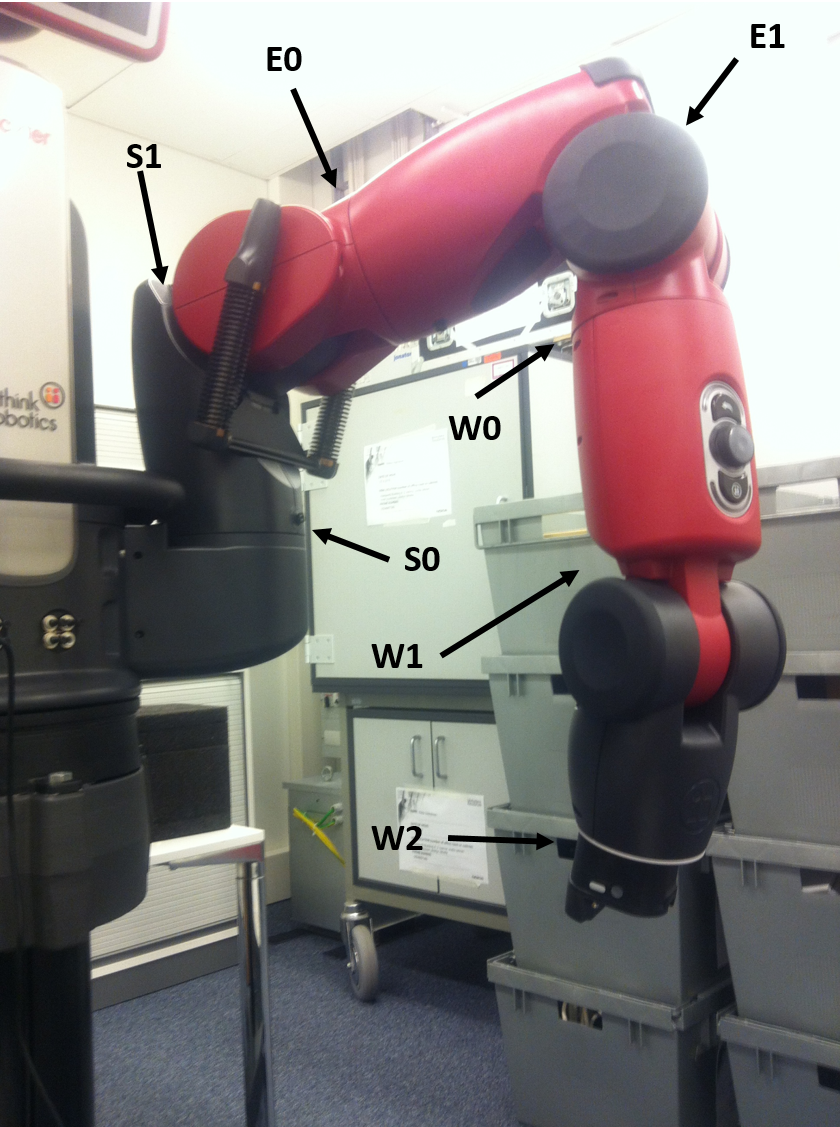
\includegraphics[scale=0.7]{baxter_arm_annotated}
\caption{This picture shows the Baxter robot and its corresponding joints. Seven degrees of freedom including shoulder roll $s_0$,  elbow roll $e_0$, wrist roll $w_0$, wrist roll $w_2$, shoulder pitch $s_1$ , elbow pitch $e_1$ and wrist pitch $w_1$ are presented on picture.}
\end{figure}
In total, Baxter's arms have fourteen degrees of freedom, which we consider as states of robot. They together form one state of the robot i.e. $(\{s^l_0, s^l_1, e^l_0, e^l_1, w^l_0, w^l_1, w^l_2\}\cup\{s^r_0, s^r_1, e^r_0, e^r_1, w^r_0, w^r_1, w^r_2\}) \in \mathbb{S}$. Then we can apply each degree of freedom an angular velocity as action, as a result, we have a set of actions $a \in \mathbb{A}$. The policy function $\pi(\cdot)$ is a $n$-layer multilayer linear neuron network that mathematically formulated as:
\begin{equation}
\pi(\vec{s}) = (f_1 \circ f_2 \cdots f_n)(\vec{s})
\end{equation} 
where $f_i(\vec{s}), \forall i \in \{1\cdots n\}$ is defined as $W_i \cdot \vec{s}$ as a single layer linear neuron network.
The transition function follows physical law with some noise. The reward function is defined similar as cart-pole problem.
Now we follow the formulation of PGPE algorithm, using two hidden parameters $\mu, \sigma^2$ for the each parameters in policy function. We also update algorithm according to PGPE algorithm ~\ref{alg:pgpe} mentioned in section Reinforcement Learning. Similarly, we also define the reward function as a step function. Only here we need to define time steps to be longer, which can be seen as Formula~
\begin{equation}
    R(s,\theta, t)= 
\begin{cases}
    0,				& \text{if} |s|\leq 0.05, |\theta| \leq 0.05, t \leq 2000\\
    -1,              & 2.4 \geq |s|\geq 0.05, 0.7 \geq |\theta| \geq 0.05, t \leq 2000 \\
    -2 \cdot (2000 - t), 		& \text{otherwise}
\end{cases}
\end{equation}

\subsection{Experiment Result Using Baxter Simulator}
Based on the Robot Operating System(ROS), several simulators supports simulation of Bater robot. One of them is Gazebo, an official simulator provided by ROS.
\subsection{Experiment Result Using Baxter Robot}



\bibliography{library}
\bibliographystyle{siam}

\end{document}
